\documentclass[twoside, titlepage, 12pt, a4paper]{article}
\usepackage[utf8]{inputenc}
\usepackage{hyperref}
\usepackage{csquotes}
\usepackage{listings}
\usepackage{float}
\usepackage{graphicx}
\usepackage{mathptmx}
\usepackage{comment}
\usepackage[
backend=biber,
style=alphabetic,
sorting=ynt]{biblatex}
\usepackage{anysize}
\usepackage[spanish]{babel}

%set style of listings
\lstset{
	language=C,
	basicstyle=\footnotesize
}

%Paragraph format
\setlength{\parindent}{2em}
\setlength{\parskip}{1em}

% color in page
\usepackage{afterpage}
\usepackage{xcolor}
\usepackage{pagecolor}

% Margin sizes for page
\marginsize{3cm}{3cm}{2.5cm}{2.5cm}
\usepackage{setspace}
\spacing{1.5}
 
\usepackage[nonumberlist, acronym]{glossaries}
\makeglossaries

\newglossaryentry{latex}
{
	name=latex,
	description={A markup language}
}


\addbibresource{bibliography.bib}
\title{Análisis y automatización de doble factor de autenticación en sistemas GNU/Linux}
\author{Roselló Morell, Sergio\\
\texttt{sergio.rosello@live.u-tad.com}}

%Making sections load on odd pages
\let\oldsection\section
\def\section{\cleardoublepage\oldsection}

\begin{document}
\begin{titlepage}
	\centering
	\begin{figure}
		\centering
		\subfloat{
\includegraphics[width=0.3\textwidth]{Media/logoU-TAD.png}}
		\qquad
		\subfloat{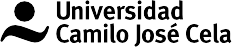
\includegraphics[width=0.3\textwidth]{Media/logoUCJC.png}}
	\end{figure}\par\vspace{1cm}
	{\scshape\Large Trabajo de fin de grado\par}
	\vspace{1.5cm}
	{\huge\bfseries Análisis y automatización de doble factor de autenticación en sistemas GNU/Linux\par}
	\vspace{2cm}
	{\Large\itshape Sergio Roselló Morell\par}
	\vfill
	\raggedright
	\textbf{Tutor:} Eduardo Arriols Nuñez\par
	\textbf{Grado:} Ingeniería en Desarrollo de Contenidos Digitales\par
	\textbf{Convocatoria:} 06.07.18\par

	\vfill

\end{titlepage}
\section*{Agradecimientos}
Debo agradecer a Eduardo Arriols, mi tutor del trabajo todo el apoyo y consejos dados. Estoy seguro de que sin su ayuda, este trabajo no hubiese llegado a su nivel actual. Durante el proceso de elección del trabajo, me ayudó a darme cuenta de lo que quería hacer exactamente y desde ese momento, no ha parado de inspirarme con distintas formas de ver las cosas. De eso, le estoy muy agradecido. No hubiese podido imaginar un tutor mejor para mi trabajo.
También quiero agradecer a la universidad el buen trabajo a la hora de escoger al personal docente de mi grado, puesto que en todo momento han demostrado más que profesionalidad y compañerismo hacia mi y mis compañeros de carrera.\par
Esta oportunidad formativa no hubieses sido posible de no ser por el esfuerzo de mis padres y mis abuelos, que, sin ninguna duda y con plena confianza en mí, incitaron y asesoraron en los momentos más decisivos de mi vida. Vosotros sois la razón por la que soy quien soy. Os estoy y estaré eternamente agradecido por eso.\par
Por último, dar las gracias a toda la gente que ha dedicado su tiempo en ayudarme a sacar la mejor versión de mi mismo en este trabajo. A nivel personal y profesional. Muchas gracias a todos.
\clearpage
\section*{Resumen}
Este documento explica al lector la experiencia que he tenido durante el periodo de realización del trabajo de final de grado. Este trabajo trata sobre el análisis en profundidad de los \gls{acr-dfa}, específicamente \gls{acr-pam} y la creación de un \gls{script} para ayudar a los usuarios menos técnicos a configurar un \gls{acr-dfa}.
Durante la fase de investigación de las tecnologías existentes, encontré algunas que ofrecían usa solución elegante, mediante \gls{dbus} pero acabando la fase de investigación encontré un proyecto llamado \gls{acr-pam} que redefinió la forma en la que planteaba el trabajo ya que es la forma por defecto de autenticar a los usuarios que tienen la mayoría de sistemas \gls{GNU/Linux}.\par 
Al iniciar el proyecto, al principio con enfoque mucho más práctico ha acabado teniendo un enfoque investigativo puesto que para entender el módulo de autenticación, he tenido que construir una base fuerte sobre la que sentirme cómodo. Sin ella, el trabajo realizado, aunque funcionalmente completo, no me hubiese sido ni la mitad de estimulante ni interesante.
\clearpage
\section*{Abstract}
This document reports my experience as i research Two Factor Authentication in \gls{GNU/Linux} and develop a script to help less technical users configure their own. \par
During the research phase, i came across several elegant implementations, all of them worked with \gls{dbus}. during the final stages of this period, i discovered \gls{acr-pam} which changed my whole perspective on this project. Most \gls{GNU/Linux} systems use this module to enable authentication for their users.\par
At the start of this project i would've expected to code a lot more, but now i realise that without a solid foundation, i may have been able to do what i had proposed, but i would not have the understanding on how the \gls{acr-pam} fits into the whole equation and the many benefits it provides. this, i think is the point of this work.
\clearpage

\spacing{0.5}
\tableofcontents
\clearpage
\listoffigures
\clearpage
\spacing{1.5}
\section{Estado del arte}
Se investigará la evolución de los ordenadores, la implicación que estos tienen en nuestra sociedad actual y las precauciones de seguridad que debemos tener al usarlos.
\subsection{Evolución de las tecnologías}
Los ordenadores forman una gran parte de nuestra sociedad desde que fueron inventados. El primer ordenador que se creó fue el Mark I, en 1944. Este ordenador estaba hecho mayoritariamente para realizar cálculos, pesaba cinco toneladas y se sobrecalentaba.
Desde Mark I, como podemos observar en la figura \ref{fig:moore}, los ordenadores han ido duplicando el número de transistores en circuitos integrados cada dos años \cite{moore}. Hasta ahora, y seguramente unos años más en adelante, podamos ver que se sigue cumpliendo la ley de Moore.
\begin{figure}[H]
    \centering
    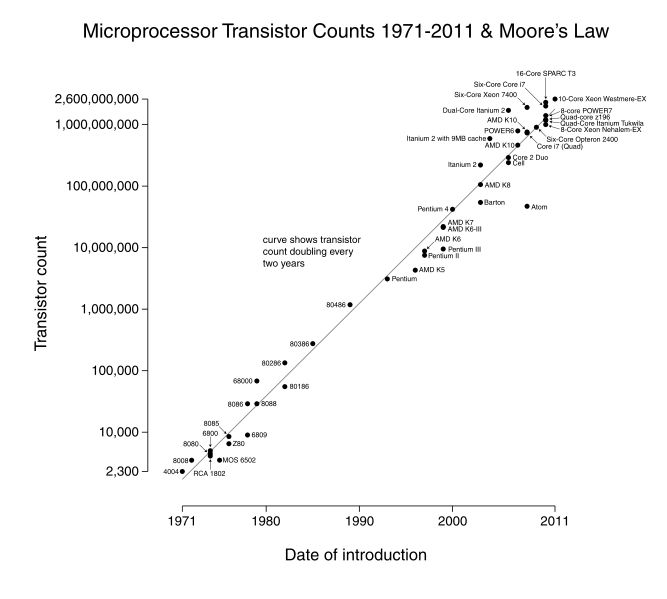
\includegraphics[width=0.7\textwidth]{Media/moore.jpg}
    \caption{Ley de Moore}
    \label{fig:moore}
\end{figure}
Durante el periodo de evolución de la informática, se pueden diferenciar cinco generaciones:
\begin{itemize}
	\item{\textbf{Primera generación: }}Estos ordenadores no se parecían en nada a los ordenadores modernos, eran extremadamente grandes y poco sofisticados. Eran estructuras tan grandes como una habitación entera y usaban válvulas termodinámicas como switches y amplificadores. Las válvulas termodinámicas generaban mucho calor así que a pesar de contar con unidades de refrigeración enormes, se sobrecalentaban muy frecuentemente.\par Para interaccionar con estos ordenadores, los programadores usaban un lenguaje conocido como \textit{Lenguaje de máquina} que era directamente interpretable por el circuito.\par Esta generación tuvo lugar entre los años 1940 y 1956.
	\item{\textbf{Segunda generación: }}Estos ordenadores se distinguen de la primera generación porque consiguen sustituir las válvulas termodinámicas por el  transistor. El cambio de válvulas a transistor implica más velocidad de cálculo y menos energía residual en forma de calor. Otra de las ventajas de los transistores es que, al ser más pequeños, reducen el tamaño del ordenador y lo hacen más económico.\par En esta generación, también se consiguió almacenar información en discos, siendo esta la primera forma de almacenamiento de información persistente.\par Esta generación tuvo lugar entre los años 1956 y 1963.
	\item{\textbf{Tercera generación: }}Se implementaron por primera vez los circuitos integrados, que contenían muchos transistores en chips semiconductores. Las ventajas de esta aportación fueron velocidad de cálculo, que aumentó mucho, el tamaño se redujo considerablemente y se continuaron abaratando los precios. En vez de Lenguaje máquina, ahora los programadores usan monitores y teclados llamados \gls{acr-tty} para comunicarse con el ordenador. Hasta esta generación, los ordenadores no estaban destinados para un uso personal. Solo las grandes empresas podían permitirse tener un ordenador.\par Esta generación tuvo lugar entre los años 1964 y 1971.
	\item{\textbf{Cuarta generación: }}Es la generación con más impacto en la sociedad. La tecnología avanzó hasta tal punto que los fabricantes podían poner miles de transistores en un único circuito integrado. En esta época se puso a la venta el Intel 4004, el primer microprocesador en venderse de forma masiva. Este desarrollo inició la industria de los ordenadores personales.\par A mediados de los 70, salieron al mercado ordenadores como el Altair 8800 que venían a piezas y su usuario tenía que construir para usar. A finales de los 70, inicios de los 80, salieron al mercado ordenadores construidos de fábrica, como el Comodore PET, Apple II y el primer ordenador IBM. Al inicio de los 90, los ordenadores personales y la capacidad de crear una red de comunicación entre ellos dio paso a la creación de Internet. Se mejoró también la capacidad de almacenamiento de los discos además de la velocidad en general. Aparecieron los primeros ordenadores portátiles, que presentaban una \gls{acr-gui} para facilitar la interacción entre el usuario y la máquina.\par Los usuarios de los ordenadores ya no tenían que ser usuarios técnicos ni debían realizar un curso de formación para saber usarlos. Esto avivó la tasa de adopción de esta tecnología enormemente.\par
		Incluso a principios de esta generación, al popularizarse tanto los ordenadores personales, ya urgía una forma de autenticación de los usuarios. A partir de esta época, se ha intentado concienciar a la población de que proteger los datos personales con una contraseña segura es la mejor forma de asegurar la privacidad de sus datos.
		Esta generación tuvo lugar entre los años 1971 y 2010. \par
	\item{\textbf{Quinta generación: }}Actualmente nos encontramos en esta generación. Algunos dicen que la adopción de los ordenadores cuánticos es el próximo gran paso, pero desde mi punto de vista, aún queda bastante para que eso ocurra.\par Creo que la quinta generación se caracterizará por el cambio de mentalidad de los usuarios de ordenadores. Hoy en día, tener la información guardada en un ordenador ya no es un privilegio, ni una ventaja competitiva. La verdadera ventaja es la disponibilidad de la información en cualquier ordenador al que te conectes, proporcionando al usuario una forma de acceso a información revolucionaria. Nunca antes ha sido posible acceder desde cualquier sitio a la información de un usuario. \par
		En la actualidad, es muy común almacenar todo tipo de información en nuestros ordenadores, incluso en nuestras cuentas on-line. Almacenamos desde imágenes hasta documentos importantes. La información almacenada en nuestros dispositivos es, por tanto, gran parte de nuestra vida. Por esta razón, es más importante que nunca proteger nuestras cuentas, tanto locales como on-line. \par
		Esta generación empezó en 2010.
\end{itemize} \par
Ha sido a partir de la cuarta generación cuando los desarrolladores de aplicaciones han tenido que preocuparse de verificar que las credenciales que usan sus usuarios son correctas. Originariamente, \gls{GNU/Linux} no tenía un método de autenticación definido. Esto significa que cada desarrollador gestionaba la autenticación del usuario de una forma distinta. Para los desarrolladores, esto significaba más tiempo perdido implementando medidas de seguridad que no guardan relación con el contenido de sus aplicaciones y para los administradores de sistemas significaba que tenían que mantener diversos métodos de autenticación (uno para cada aplicación) actualizados para seguir cumpliendo los estándares de seguridad deseados. \par
Existían dos prácticas para realizar la autenticación del usuario, la primera consiste en buscar los nombres y hashes de los usuarios en los archivos \textit{/etc/passwd} y \textit{/etc/shadow} y compararlo con lo que había introducido el usuario. La segunda mentalidad directamente gestionaban la autenticación de la forma que querían. \par
Como era de esperar, al no haber ni estándar ni protocolo, urgía una solución rápido. En 1995, \gls{Sun} propuso un mecanismo llamado \gls{acr-pam}. Este mecanismo proporcionaba a los desarrolladores de aplicaciones una \gls{acr-api} que se ocupaba de manejar la lógica de autenticación y beneficiaba al administrador de sistemas porque unificaba el control de autenticación en un solo sitio, que además, permitía implementar distintos esquemas de autenticación.
\subsection{Consecuencias de la evolución}
El rápido desarrollo de esta tecnología, como era de esperar cuando las cosas se hacen rápido y a contra reloj, introdujo un factor de error en la ecuación. Desde los inicios, ya sea por fallo humano o casualidad, se habla de un fenómeno llamado \textit{\gls{bug}}. Este término forma parte de la jerga informática desde 1947, año en que, durante el ensamblaje del ordenador \textit{Harvard Mark II}, tras el incorrecto funcionamiento del ordenador, los ingenieros revisaron las conexiones del ordenador y se encontraron con un insecto que adherido a dos cables, provocaba el fallo en el sistema. Desde entonces, se llama \textit{\gls{bug}} al fallo en un programa, ya sea lógico o sintáctico.\par
Debido a la rápida adopción de los ordenadores por la población, las compañías debían sacar los productos rápido y no tenían tiempo a arreglar algunos \textit{\gls{bug}s}. Un estudio realizado por el \textit{\gls{acr-nist}} concluyó en que los fallos en el software le cuestan a la economía estadounidense 59.5 billones de dólares anuales.\cite{NIST} Esto es un fenómeno imposible de evitar ya que en definitiva el software lo escriben seres humanos y nosotros, al ser seres imperfectos, no podemos producir software perfecto. Siempre hay algo que se nos escapa.\par
A medida que más usuarios usan programas, se van encontrando nuevos fallos, que dependiendo de la escala de gravedad podrían ser críticos, tanto para las empresas como para sus usuarios ya que si un usuario con malas intenciones encuentra un fallo de seguridad en la aplicación, dependiendo de su gravedad, podría, en teoría obtener información sensible de otros usuarios además de información interna de la compañía que ha hecho el software.\par
Para combatir este problema, algunas empresas han decidido recompensar a los usuarios que encuentran estos fallos. Al ofrecer una recompensa económica, la empresa incita al usuario a describir el fallo para que se pueda arreglar. Este tipo de programa se llama \gls{acr-bbp}. Existen varias páginas que se dedican a gestionar las ofertas de las empresas y los hallazgos de los usuarios para que ambos salgan ganando.\par
Hoy en día, tenemos todos nuestros datos \textit{on-line}. Esto nos ofrece grandes ventajas como el acceso inmediato a nuestra información personal pero corremos un gran riesgo al confiar en las empresas que hacen que esto sea posible porque no existen programas sin  \textit{\gls{bug}s}.
\subsection{Necesidad de seguridad}
A medida que ha ido evolucionando la tecnología, medidas de seguridad previamente válidas, han ido quedando deprecadas debido a fallos que se han encontrado en los protocolos o nuevas versiones de estas mismas. El campo de la seguridad en la informática ha ido evolucionando como si se tratara del juego del ratón y el gato en el que los desarrolladores arreglan e inventan nuevas formas de proteger la información de los usuarios y los hackers vulneran esas implementaciones.\par Ahora mismo, los usuarios son los que más tienen que perder. Tenemos todos nuestros datos almacenados en servidores de grandes empresas como Google o Facebook y en el caso de que se filtre nuestra información al mundo, tanto fotos personales como documentos sensibles se verían expuestos a todos los usuarios de Internet.\par Para evitar esto, estas empresas implementan métodos de seguridad cada vez más avanzados como el doble factor de autenticación para iniciar sesión en la cuenta.\par Las medidas de seguridad que proporcionan las empresas como Google o Facebook son bastante buenas pero no son suficientes. Tampoco podemos pedir a estas empresas que implementen todo tipo de sistemas de autenticación de usuarios, ya que al final, tienen que hacer el proceso fácil y sencillo para que le gente quiera y sepa usarlo.\par Podemos aumentar la seguridad de nuestro sistema configurando nosotros mismos las distintas formas de autenticarnos en nuestros sistemas. Una de las formas en las que podemos aumentar la seguridad de nuestro sistema es mediante el \gls{acr-dfa}. Algunos ejemplos de esta implementación son:
\begin{itemize}
	\item Contraseña + Llave USB
	\item Contraseña + App generadora de códigos (Google Authenticator)
	\item App generadora de códigos + Sensor de huella dactilar
	\item Contraseña + Sensor de retina
\end{itemize}
A cuanto más valor, ya sea económico o emocional, más medidas de seguridad serán implementadas en proteger dicha información.\par
En definitiva, es muy complicado tener un entorno seguro en el que poder confiar porque muchos de los vectores de ataque no dependen del usuario final, sino de terceros (tantos como distintos servicios use el usuario). Es importante tener un buen nivel de seguridad en todos los dispositivos, pero este no debe interponerse entre las tareas que un usuario tiene que hacer en su ordenador ya que de lo contrario, sería un inconveniente, no una ventaja. Cada usuario debe establecer el grado de seguridad de sus cuentas, tanto en Internet como de sistema.\par
Para la mayoría de usuarios, una contraseña, aunque menos segura que un \gls{acr-dfa} será más conveniente porque la naturaleza de la información que tiene que proteger no es tan importante como para asegurar su confidencialidad.
\clearpage
\clearpage
\section{Introducción}
En esta sección se presenta mi experiencia con la tecnología y como ésta ha derivado en este trabajo. Además, se expone la envergadura de este documento y las competencias adquiridas en la realización del proyecto.
\subsection{Motivación}
Desde pequeño, mi interés por los ordenadores era más que evidente. Recuerdo aún la forma en la que miraba el símbolo de sistema de Windows 7 pensando: \textit{Ojalá supiera como funciona esto}. Siempre ha existido ese interés por el software en mí. Entender como funciona, desde el programa más básico al más complicado, ha sido siempre la fuerza de atracción hacia este mundo. Al decidir dedicar mi vida profesional a ello, decidí iniciar mi formación con un grado universitario.
Como todo alumno de primero de carrera, inicié el curso con ganas y Windows.\par
Durante el transcurso de la carrera, se hacía evidente que Windows no era el mejor sistema operativo para hacer las prácticas. Durante el primer curso usé una máquina virtual con \gls{Ubuntu} para hacer las prácticas. Cuando vi que usaba más la máquina virtual que el sistema operativo sobre la que corría, supe que era hora de dejar atrás Windows. El primer sistema operativo que instalé fue \gls{Ubuntu} y durante unos años dediqué mi tiempo libre a aprender a gestionar el sistema por comandos. Esto me llamaba la atención enormemente. Cuando me sentí lo suficientemente cómodo para cambiar nuevamente de sistema operativo, decidí cambiar a \gls{Arch linux} aunque primero debía pasar por \gls{Manjaro}, una distribución basada en \gls{Arch linux}, más sencilla de utilizar, pero con el mismo sistema por debajo. Cuando finalmente me vi capaz de pasar a \gls{Arch linux} y lo configuré correctamente, sentí que todos los años de aprendizaje habían llevado a buen puerto. \par
Todo el proceso de aprendizaje que he pasado durante estos años me ha servido para aprender y valorar el sistema operativo. Esta es la razón por la que supe desde el primer momento en que nos dijeron que fuésemos pensando sobre que queríamos hacer el trabajo de fin de grado que quería hacerlo sobre \gls{GNU/Linux}.\par
Tras toda esta experiencia, he querido ampliar mis conocimientos en \gls{GNU/Linux}. Durante la reunión con mi tutor, vimos algunas opciones de investigación y finalmente, al estar interesados en la seguridad de las aplicaciones y sistemas, decidimos que era buena idea indagar por esa rama.\par
Durante el transcurso de la carrera, ya sea por requisito de los profesores o por mis proyectos personales, he sido un gran usuario del sistema de control de versiones, \gls{Git}. Lo he usado desde prácticas en las que era necesario hasta para este mismo documento. Desde que empecé a usarlo, vi que no se trataba simplemente de una herramienta para gestionar mis proyectos, sino de un estilo de vida, una forma de enseñar y compartir los proyectos en los que estás involucrado.\par
La mayor parte de los programas que uso en mi sistema operativo se desarrollan de forma abierta en los que puedes ver el progreso y interaccionar con los desarrolladores, incluso ayudarles a detectar errores o solicitar un \textit{pull request} para arreglar algún fallo.\par
Espero que el resultado de este proyecto consiga reducir el nivel técnico mínimo necesario para configurar un \gls{dfa}, bastante más seguro que cualquier sistema por defecto.\par
Cualquier usuario, técnico o no, debería tener fácil acceso a varias formas de verificar su identidad. Según estas, ya es éste, quien puede decidir cual usar, pero al menos, el usuario tiene la opción de elegir.
\subsection{Descripción del proyecto}
Este proyecto consta de dos partes coexistentes. Una parte de investigación sobre las distintas formas de autenticación en sistemas \gls{GNU/Linux} y una parte práctica.\par
La meta inicial del proyecto era desarrollar un sistema de \gls{acr-dfa} para dichos sistemas pero al descubrir durante la fase de investigación que ya existía, se cambió de perspectiva ya que no tenía sentido plantear un mecanismo de autenticación superior al de los expertos desarrolladores que implementaron \gls{acr-pam} en 1995. Como consecuencia de este descubrimiento se decide implementar un \gls{acr-dfa} para demostrar los pasos a seguir en su desarrollo pero se encontró un proyecto\footnote{\url{https://github.com/ColumPaget/pam_usbkey}} en \gls{GitHub} que hacía exactamente lo que tenía pensado implementar. Tras encontrar dicho proyecto se cambió de perspectiva. Se decidió desarrollar un \gls{script} en \gls{acr-bash} que facilitase al usuario no técnico la configuración del módulo \gls{acr-usb} para \gls{acr-pam}.\par
El \gls{script} que he creado ayuda al usuario a seleccionar el \gls{acr-usb} que quiera usar, le explica las diferencias entre las distintas formas que hay de configurar el Módulo y le deja decidir donde quiere introducir la línea de configuración ya que al ejecutar las órdenes de forma secuencial, dependiendo de la posición en la que se coloque la línea, el módulo hará una cosa o otra. \par
Previo a el \gls{script}, para configurar el módulo \gls{acr-usb}, el usuario debía leer la documentación oficial de PAM para averiguar que archivo es el que debe configurar y como lo debe hacer. Lo que se consigue con el \gls{script} es reducir la curva de aprendizaje necesaria para configurar un método de autenticación más seguro que el de la contraseña por defecto. Esto hará que más usuarios tengan acceso a mejor autenticación en sus ordenadores sin que pierdan conveniencia y comodidad.
\subsection{Competencias adquiridas}
Al acabar cualquier tarea propuesta en la vida, uno siente una sensación de realización fuertemente vinculada con esta. Además de realización, si uno se para a analizar, se da cuenta de las distintas aptitudes y actitudes desarrolladas, de forma involuntaria tras la realización del proyecto. En el caso de este proyecto, siento que he reforzado y desarrollado las siguientes.
\subsubsection{Aptitudes adquiridas o reforzadas}
A continuación presento una lista de las aptitudes que más he desarrollado durante la realización del proyecto.
\begin{itemize}
	\item{\textbf{\gls{acr-bash}}}\par Decidí usar este lenguaje de programación para hacer el \gls{script} porque sabía que no me iba a encontrar con complicaciones a la hora de asegurar que funcione en cualquier equipo ya que todos los programas usados en el script vienen instalados de forma predeterminada en la gran mayoría de sistemas.
	\item{\textbf{\gls{C}}}\par \gls{acr-pam} está escrito en \gls{C} y he tenido que leer y entender como funciona el submódulo \gls{acr-usb} para ver como se comunican ambos módulos.
	\item{\textbf{\gls{Python}}}\par En la primera implementación que hice, usé este lenguaje de programación para bloquear la pantalla del ordenador mediante \gls{dbus}.
	\item{\textbf{\gls{Linux}}}\par Durante el transcurso del proyecto he estado investigando el funcionamiento de \gls{Linux} aunque más detalladamente en los mecanismos de autenticación de usuarios que tiene.
\end{itemize}
Las siguientes dos aptitudes, aunque indirectamente relacionadas con la realización del proyecto, han sido directamente relacionadas con la realización de este documento por tanto, las incluyo en el documento.
\begin{itemize}
	\item{\textbf{\gls{Vim}}}\par Este documento ha sido escrito completamente en \gls{Vim}. La extensión de este documento ha servido para aprender tanto funciones básicas como funciones avanzadas de \gls{Vim}
	\item{\textbf{\LaTeX{}}}\par Al igual que en el caso de \gls{Vim}, la complejidad de este documento ha servido para desarrollar un mejor entendimiento de este sistema de composición tipográfica.
\end{itemize}
\subsubsection{Actitudes adquiridas o reforzadas}
La mayor parte de estas actitudes las he desarrollado en otros proyectos y ya sabía que era capaz de demostrarlas. La última, sin embargo me ha sorprendido reconocer que la poseo.
\begin{itemize}
	\item{\textbf{Resolutivo}}\par Durante la primera iteración de investigación/implementación, encontré una forma de desbloquear el equipo mediante \gls{dbus}. Esta forma, aunque funcional, no es elegante. Es más parecido a un ``hack" que a una solución elegante y segura. Si no hubiese ``dado un paso atrás", no hubiese continuado investigando/implementando otras soluciones. \par Cuando encontré PAM\_USB, me obcequé en hacer que funcionase, ya que si no funcionaba, no podía avanzar en el trabajo. De nuevo, tuve que dar un paso atrás para buscar otras implementaciones para el módulo \gls{acr-pam} con \gls{acr-usb}.\par
		Esta actitud la he tenido que trabajar mucho ya que no es raro en mí centrarme mucho en un punto y no observar las alternativas.
	\item{\textbf{Persistencia}}\par Guarda una relación directa con la forma en la que he enfocado el trabajo. Desde su primera fase a la última, he sido constante en el desarrollo del proyecto.
	\item{\textbf{Adaptabilidad}}\par Durante toda mi vida de estudiante, mi forma de retener la información y por consiguiente aprender, ha sido escuchando al profesor. Leer los apuntes a mi me sirve como refuerzo a la explicación del profesor. Durante este proyecto, no he seguido esa misma dinámica, ya que no he tenido un profesor a quien escuchar, he tenido que investigar y formarme a base de la lectura de las páginas de documentación y los comentarios informativos en el código.
\end{itemize}
\subsection{Estructura del documento}
Este documento está compuesto por varias secciones. Cada una aporta una visión necesaria para proporcionar unidad al proyecto.
\begin{enumerate}
	\item{\textbf{Estado del arte}}\par
		En este apartado se describe la evolución de los ordenadores, poniendo en contexto de esta forma la importancia de los mecanismos de autenticación en relación a los usuarios de los mismos y los tiempos modernos.
	\item{\textbf{Introducción}}\par
		Se redactan las fuerzas mayores que han desencadenado en la realización de este proyecto además de una breve descripción del proyecto y las aptitudes y actitudes desarrolladas a consecuencia de él.
	\item{\textbf{Objetivos}}\par
		Análisis de los objetivos generales y específicos propuestos durante el desempeño del proyecto.
	\item{\textbf{Métodos de trabajo}}\par
		Observación de la forma en la que se ha trabajado. Breve explicación de la misma, ventajas e inconvenientes y esquema general de los pasos realizados durante el proyecto.
	\item{\textbf{Investigación y resultados}}\par
		Esta sección consta de dos partes principales. Una de investigación y otra de Desarrollo. En la primera, se hace una investigación general de las distintas formas de autenticación disponibles tanto a usuarios como a administradores de sistemas de grandes redes de ordenadores. Tras el análisis, se explica por qué se decidió optar por \gls{acr-pam}, sus ventajas e inconvenientes relacionadas con las formas previamente analizadas y se procede a explicar en detalle dicho módulo. Una vez analizado el módulo, se explica como sería el proceso de creación de un sistema \gls{acr-pam}, se explican las distintas formas existentes de usar un módulo \gls{acr-pam} para demostrar su adaptabilidad. El segundo apartado contiene el análisis de las distintas pruebas realizadas con sistemas con la misma finalidad y finalmente el análisis, estructura y desarrollo del \gls{script} que se ha creado para ayudar a normalizar este mecanismo de autenticación.
	\item{\textbf{Conclusiones}}\par
		Una vez expuesto todo el contenido del proyecto, se llega a una conclusión del proyecto además de posibles formas de expandir el trabajo hacia el futuro.
\end{enumerate}
\clearpage
\section{Objetivos}
El presente punto tiene como finalidad describir tanto los objetivos generales como específicos del proyecto. Los objetivos están ordenados de generales a específicos.
\begin{itemize}
	\item{\textbf{Expandir mi conocimiento sobre \gls{GNU/Linux}}}\par
		Además de ser un sistema operativo versátil y fehaciente, es una prueba viviente de que se puede hacer código libre en comunidad y de calidad.
	\item{\textbf{Contribuir a la comunidad de desarrolladores con alguna aportación}}\par
		Durante la investigación y desarrollo del trabajo de fin de grado, he aprendido sobre las distintas tecnologías gracias a los manuales oficiales de \gls{acr-pam}. Esto, como debería ser, es software y documentación disponible a cualquier persona, con una licencia GNU General Public License que: garantiza tu libertad de distribuir y cambiar todas las versiones de un programa para asegurar que permanece libre para todos sus usuarios. \cite{GNU-GPL} \par
		Creo que se debería contribuir a la comunidad de desarrolladores en general, además, si puedo beneficiar a alguien con el documento o código generado durante este trabajo, quedo más que satisfecho.
	\item{\textbf{Investigar ámbito de seguridad}}\par
		Se decidió que la investigación debía ser en el ámbito de seguridad porque tanto a mi tutor como a mi nos interesaba la idea.
	\item{\textbf{Investigación y análisis del \gls{acr-dfa} en \gls{GNU/Linux}}}\par
		Se decide ahondar en el ámbito tras ver un vídeo en el que se presentaba un mecanismo para evitar la fase de autenticación en un sistema operativo basado en \gls{GNU/Linux}. La clave estaba en el uso de una herramienta pre-instalada para enviar mensajes a las aplicaciones encargadas de autenticar la identidad de los usuarios informándolas de que el usuario ya estaba autenticado. Estas herramientas no estaban monitorizadas por los administradores de sistemas debido al gran volumen de información que pasa a través de ellas.
	\item{\textbf{Crear un sistema \gls{acr-dfa}}}\par
		El objetivo inicial en este trabajo era crear un sistema que permitiese al usuario bloquear y desbloquear el ordenador con un \gls{acr-usb}. Cuando se empezó a investigar las distintas formas de hacer esto, el primer paso lógico era centrarse en \gls{dbus} ya que existían proyectos que conseguían este objetivo. Tras el primer ciclo de investigación/implementación conseguí bloquear el sistema al enviar un comando mediante \gls{dbus} al programa que se encarga de bloquear el sistema pero debido a varios factores que se explicarán más adelante, no era una solución buena. \par 
	\item{\textbf{Desarrollar un módulo \gls{acr-pam} para la autenticación mediante \gls{acr-usb}}\par
		Tras una investigación inicial, se descubrió que esta librería es la forma por defecto de autenticación de usuarios en la mayoría de sistemas \gls{GNU/Linux}. Su diseño contemplaba la posibilidad de utilizar múltiples factores de autenticación. Para avanzar, ahora se debía entender como funcionaba \gls{acr-pam} y como crear un módulo de autenticación por \gls{acr-usb} que lo implementara.
	\item{\textbf{Desarrollo de \gls{script} para facilitar adopción}}\par
		 El cauce de este proyecto se centró en facilitar la adopción de este módulo a los usuarios, de forma que más gente no técnica pueda acceder a mejor autenticación. Esto se consigue creando un \gls{script} que al ejecutarlo se encargue de la parte más complicada del proceso de instalación de un \gls{dfa}: la configuración, ya que si se configura erróneamente, existe la posibilidad de que el usuario se quede bloqueado fuera de su ordenador.\par
	 \item{\textbf{Elección del lenguaje para el \gls{script}}}\par
		El siguiente objetivo fue la elección del lenguaje. Al elegir lenguaje de programación para el \gls{script} tuve en cuenta varios factores. Conocimiento actual del lenguaje, complejidad de implementación en dicho lenguaje, disponibilidad de dicho lenguaje en los posibles sistemas donde se use \gls{acr-pam} y en caso de no haber usado el lenguaje previamente, curva de aprendizaje del mismo. Finalmente, el lenguaje de programación usado ha sido \gls{acr-bash} debido a que su integración con \gls{GNU/Linux} es excelente, la curva de aprendizaje no era exagerada y que es compatible con todos los sistemas en los que funciona el módulo.
	\item{\textbf{Enumeración de dispositivos \gls{acr-usb} conectados al sistema}}\par
		Una vez escogí \gls{acr-bash}. Debía averiguar como usarlo para encontrar los dispositivos \gls{acr-usb} en el sistema.\par
\end{itemize}

\clearpage
\section{Métodos de trabajo}
Durante el desarrollo del proyecto, he seguido una metodología de desarrollo ágil, ya que a mi parecer, es la forma más eficiente de trabajar en un proyecto. Comparada con el desarrollo en cascada, aporta muchas ventajas al flujo de trabajo. \par
En esencia, las metodologías ágiles son una evolución de la conocida implementación en cascada ya que generalmente se consiguen mejores proyectos, mayor satisfacción del cliente y mayor unión entre los miembros del equipo de desarrollo y el cliente.
\begin{figure}[H]
    \centering
    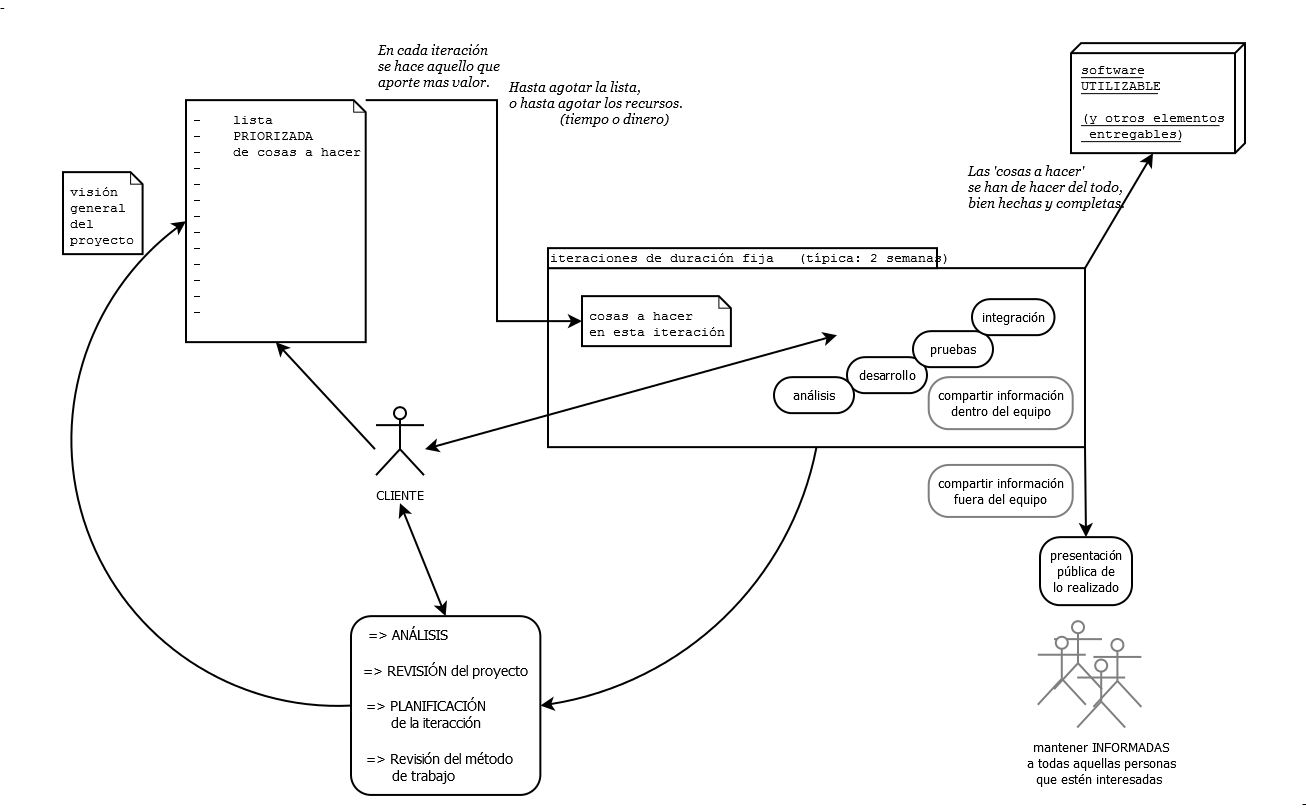
\includegraphics[width=1\textwidth]{Media/agile.png}
    \caption{Diagrama explicativo de una Metodología ágil}
    \label{fig:agileMethodology}
\end{figure}
Esta metodología se basa en una serie de ideas que quedan bien plasmadas en su manifiesto. Esto es, aunque valoramos los elementos de la derecha, valoramos más los de la izquierda.\cite{agile} 
\begin{itemize}
	\item{\textbf{Individuos e interacciones} sobre procesos y herramientas}
	\item{\textbf{Software funcionando} sobre documentación extensiva}
	\item{\textbf{Colaboración con el cliente} sobre negociación contractual}
	\item{\textbf{Respuesta ante el cambio} sobre seguir un plan}
\end{itemize}\par
Las ventajas de este estilo de desarrollo frente a estilos más conservadores como el de cascada son, entre otras, que el cliente trabaja con el equipo de desarrollo constantemente para adaptar el producto a las características deseadas, el flujo de trabajo se basa en la repetición de actividades como análisis de requisitos, diseño, implementación, testeo y producción de forma iterativa hasta conseguir un producto acabado.\par
Diría que he seguido bastante de cerca el estilo de desarrollo propuesto por esta metodología. Durante el periodo de desarrollo del trabajo, he mantenido una relación cercana con mi tutor, manteniéndole siempre al día sobre los progresos del proyecto, cada semana aproximadamente nos reuníamos para ver el estado del proyecto, en la que le describía los progresos prácticos conseguidos. Cuando decidimos que \gls{dbus} no era una buena solución, supe responder al cambio y adaptar el proyecto a nuevas y mejores soluciones. \par
A medida que avanzaba el proyecto, el área de investigación se volvía más pequeña y enfocada. Durante las primeras semanas, me centré en investigar el transcurso de los métodos de autenticación. Una vez analizadas las distintas formas de autenticación, profundicé en \gls{dbus}, implementé un programa que enviaba un mensaje mediante este bus al programa encargado de bloquear y desbloquear el sistema y conseguí bloquear el sistema. Esto me servía como prueba de concepto pues, si había logrado bloquear, solo faltaba añadir una capa de abstracción más que enviase el comando de bloqueo si las acciones del usuario cumplían con el comportamiento esperado. \par
Durante el periodo de investigación de dispositivos con los que podía realizar un \gls{acr-dfa} llegué a la conclusión de que en realidad cualquier dispositivo hardware es válido. Cuando alguien piensa en \gls{acr-dfa}, lo más común es pensar en las aplicaciones como Google Authenticator. Lo siguiente que viene a la mente es usar una llave \gls{acr-usb} como segundo factor de autenticación, pero la realidad es que se pueden usar todo tipo de dispositivos, algunos ejemplos son: auriculares (comprobando que se complete un patrón como por ejemplo insertar y extraer el jack de audio dos veces seguidas), una tarjeta de red \textit{\gls{wifi}} (comprobando  el \textit{\gls{fingerprint}} de los dispositivos que emiten una señal \textit{\gls{wifi}} con una lista de \textit{\gls{fingerprint}s} aceptados) o cualquier módulo \gls{bluetooth} (comprobando el \textit{\gls{fingerprint}} contra una lista de \textit{\gls{fingerprint}s} aceptados). Solamente es necesario que el sistema operativo lo reconozca. \par
Finalmente, tras investigar las ventajas e inconvenientes de varios dispositivos hardware, me decanté por el \gls{acr-usb} como segundo método de autenticación. Aunque otros dispositivos como auriculares pasan desapercibidos, el sistema de verificación no puede interactuar con ellos y aunque no sea un requisito, el hecho de poder interactuar con el \gls{acr-usb}, me proporciona más formas de verificar al usuario.
\clearpage
\section{Investigación y resultados}
Durante el desarrollo de esta sección se han investigado todas las técnicas de autenticación de usuarios encontradas para \gls{GNU/Linux}. Sin estos conocimientos no hubiese quedado contento ya que aunque se hubiese podido hacer un mecanismo para iniciar sesión pero no se hubiese entendido ni la filosofía ni la comunidad detrás de \gls{GNU/Linux}. \par
En esta sección, se describen las distintas tecnologías de autenticación existentes, los problemas actuales de esas tecnologías, se defenderá la necesidad de una seguridad más agresiva, tanto para los usuarios normales como para las grandes empresas y se desglosarán las distintas formas de conseguir esta seguridad actualmente. Además, se describirá en detalle como funciona \gls{acr-pam}, desde el punto de vista del desarrollador de aplicaciones, del administrador de sistemas y del desarrollador de módulos. Se describirán las distintas formas de autenticación probadas, desde el uso de \gls{dbus} hasta el uso de \gls{acr-pam} con \gls{act-usb} sus ventajas e inconvenientes.
\subsection{Comunidad}
Al saber que quiero aportar el script y las partes del trabajo que puedan resultar útiles a la comunidad, se ha hecho una investigación para averiguar donde y como se debería subir el contenido. Ahora mismo, el núcleo de la comunidad de software abierto está en \gls{GitHub} pero existen otros sistemas distribuidos de control de versiones como GitLab o BitBucket.\par
Durante el desarrollo del proyecto, durante la búsqueda de información relacionada con \gls{acr-pam} me he encontrado con escasa información de calidad en español, por eso, y siguiendo la filosofía de libertad de documentación y software, me gustaría publicar partes de este documento para facilitar el entendimiento de \gls{acr-pam} a compañeros de habla española.
\subsubsection{Publicación del \gls{script} a \gls{GitHub}}
Para subir el \gls{script} a \gls{GitHub} se debe de tener una cuenta en la plataforma. El segundo requisito que se debe cumplir es tener un cliente git descargado en el sistema. Puede ser un cliente por consola o un cliente gráfico como GitKraken o SourceTree. Al ser un sistema de control de versiones, es preferible que todos estos pasos se realicen antes de empezar con el \gls{script}. De esta forma, además de contribuir a la comunidad, el proyecto queda controlado por versiones, ayudando al desarrollador a mantener un registro de los cambios que se han hecho en el proyecto.\par
Una vez está todo configurado, en \gls{GitHub} se crea un proyecto, se decide cual será su nombre, licencia y demás características. Cuando el proyecto ya está creado, se selecciona la herramienta escogida para comunicarse con \gls{GitHub} y se \textit{clona} el proyecto. Esto es similar a descargar el proyecto al ordenador donde se quiere realizar el mismo. Al hacer esto, se pueden ver en la herramienta seleccionada cada uno de los archivos existentes en el directorio \textit{clonado}. A partir de ahora, todos los archivos que se incluyan dentro del directorio \textit{clonado} se controlarán y se tendrá la posibilidad de crear un \textit{commit}.\par
Al crear un \textit{commit}, se copia el contenido del directorio y se envía a \gls{GitHub}. En este momento, los archivos en el directorio y los archivos en \gls{GitHub} son idénticos. Esta es la base de Git.\par
\gls{Git} fomenta el trabajo en equipo porque permite que varias personas trabajen en el mismo proyecto en distintas cosas para posteriormente hacer un \textit{merge} o fusionar el trabajo de todos.\par
Durante el desarrollo del \gls{script}, se ha usado \gls{GitHub} para controlar el desarrollo del \gls{script}\footnote{\url{https://github.com/SergioRosello/PAMHelperScript}}.
\subsubsection{Publicación de la documentación de la memoria}
Para publicar la memoria, se investigaron varias formas de hacerlo porque no se sabía exactamente cual sería la mejor. Estas tres formas son las más relevantes y variadas de las analizadas en la fase de investigación para publicar la documentación.
\begin{itemize}
	\item{\textbf{GitHub Pages}:}\par
		Este mecanismo está directamente integrado con \gls{GitHub}. Se dedica una rama del proyecto a la documentación. El inconveniente de esto es que mi proyecto de \gls{GitHub} no guarda relación directa con la documentación. Ésta no explica como funciona el \gls{script} sino como funciona \gls{acr-pam}.
	\item{\textbf{Blog personal}:}\par
		Aunque es una buena opción, para que el documento tuviera visibilidad, el blog tendría que ser popular. Eso es algo de lo que no se dispone en esta instancia.
	\item{\textbf{Medium}:}\par
		Es una plataforma relativamente nueva dedicada a documentos de cualquier clase. Lo interesante de esta plataforma es que recomienda artículos al usuario según sus gustos e intereses. Al ser una plataforma nueva a la que cada día se registran más usuarios, el público objetivo al que pueda llegar el trabajo es superior al de las otras dos alternativas. Para subir la documentación a la plataforma, simplemente es necesario adaptarla ligeramente al modelo que propone la plataforma, ponerle un título y 5 \textit{tags} que describan el contenido del documento.
\end{itemize}
\subsection{Análisis de sistemas de autenticación en sistemas \gls{GNU/Linux}}
La parte de análisis es fundamental para conocer los métodos existentes actualmente para autenticar a usuarios. Sin este análisis inicial, hubiese sido mucho más complicado realizar el proyecto debido a que el desconocimiento de las distintas formas de autenticación no me hubiese llevado a poner a \gls{acr-pam} en perspectiva. \par
La forma en la que se autentica la identidad de los usuarios de sistemas ha ido evolucionando desde que se vio que era necesaria. A continuación se exponen las formas más populares de gestión de usuarios y credenciales, tanto en el ámbito empresarial, como en el ámbito personal.
\subsubsection{Inicios de la gestión de permisos}
Cada objeto tiene asociada una tabla de 9 bits, los tres primeros indican los privilegios de lectura, escritura y ejecución del usuario que posee el objeto. Los tres siguientes son para la lectura, escritura y ejecución de los usuarios pertenecientes al grupo que posee el objeto y los tres últimos son de lectura, escritura y ejecución de los usuarios que no pertenecen a ninguno de las dos primeras categorías. Esta categoría se llama \textit{others}. Además de estos 9 bits, también pueden incluir el \gls{SetUid}, \gls{SetGid} y el \gls{StickyBit}. A pesar de ser un sistema muy simple de gestionar privilegios, cumple la mayoría de escenarios posibles en sistemas \gls{GNU/Linux} e incluso a día de hoy, se sigue usando en todos los sistemas \gls{GNU/Linux} ya que proporciona una forma sencilla y eficiente de visualizar los privilegios de los objetos y modificarlos. Esta forma de gestionar los privilegios de los objetos se puede denominar \gls{acr-acl}.
\begin{figure}[H]
    \centering
    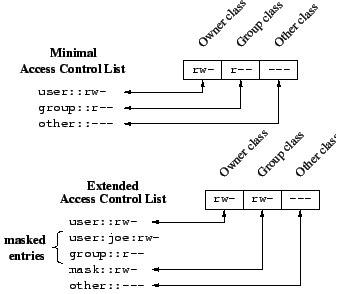
\includegraphics[width=0.4\textwidth]{Media/ACL.jpg}
    \caption{\gls{ACL}}
    \label{fig:ACL}
\end{figure}
\subsubsection{\gls{RBAC}}
Este esquema de seguridad está diseñado para organizaciones o sistemas en los que van a interactuar distintos usuarios con una gran cantidad de datos. El sistema defiende que, en lugar de tener una tabla por cada objeto, definiendo la forma que tienen los usuarios de interactuar con él, se deberían establecer una serie de transacciones, que dependiendo del rol serán distintas. Estas transacciones, una vez definidas cambian poco porque un usuario específico va a usar unos documentos específicos, dependiendo de la responsabilidad que tenga en la organización. En la figura \ref{fig:RBAC} se puede ver claramente como dependiendo del rol se va a poder acceder a ciertos objetos.
\begin{figure}[H]
    \centering
    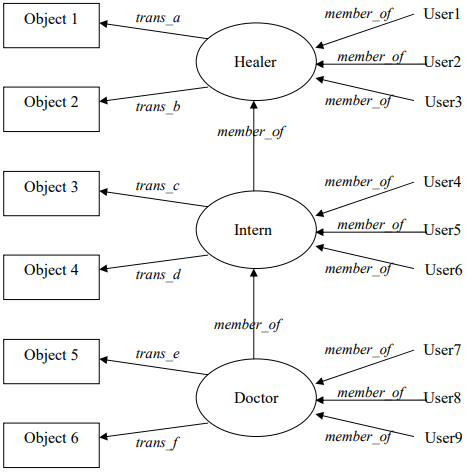
\includegraphics[width=0.5\textwidth]{Media/RBAC.PNG}
    \caption{\gls{acr-rbac}}
    \label{fig:RBAC}
\end{figure}
Dos de las ventajas de este sistema son que cumplir el principio de menor privilegio es relativamente sencillo, ya que se puede conseguir no proporcionándole  al usuario más transacciones de las que debe tener. La otra ventaja innata de \gls{RBAC} es la separación de deberes. Esto es: En el caso de tener que realizar una transferencia bancaria, nunca se debería poder proporcionar al mismo individuo el control de todo el flujo, ya que se le está dando la oportunidad de cometer algún tipo de irregularidad. Con RBAC puedes asignar dos transacciones, una que permita a un usuario solicitar una transferencia y otra que permita a un usuario validar la transferencia.
\subsubsection{\gls{LDAP}}
Este protocolo está diseñado para permitir acceso a directorios complacientes con el estándar \gls{X500} \textit{Directory Access Protocol} a sus usuarios. Uno de varios protocolos que tiene una aplicación para autenticarse con el fin de acceder al directorio \gls{X500}\cite{LDAP}. La forma de acceder a los datos cambia según el protocolo de acceso a \gls{X500}. Por ejemplo, en esta implementación, la forma de acceder a los datos sería:
\begin{lstlisting}
	cn=Rosanna Lee, ou=People, o=Sun, c=us
\end{lstlisting}
mientras que la implementación de Microsoft sería:
\begin{lstlisting}
	/c=us/o=Sun/ou=People/cn=Rosanna Lee
\end{lstlisting}
Cada uno de estos protocolos define una forma de buscar en \gls{X500} información. Podemos ver que la implementación de \textit{\gls{acr-ldap}} está ordenada de derecha a izquierda, separada por el carácter (,) mientras que la implementación de Microsoft, \gls{acr-mad} está ordenada de izquierda a derecha y separada con el carácter (/).
Aunque no sea un método de autenticación que sucede en el mismo sistema, me parece que es lo suficientemente interesante como para incluirlo ya que es un ejemplo de autenticación en red.
\subsubsection{\gls{acr-sasl}}
Es un protocolo que proporciona métodos de añadir autenticación a protocolos de red mediante identificación y autenticación de los usuarios conectados al servidor. Además, gestiona el nivel de seguridad que se desea establecer para las futuras interacciones entre el servidor y el usuario conectado. Si se llega a la conclusión de que si que se requiere una capa de seguridad, ésta se añade entre el propio protocolo y la conexión.\cite{rfc2222} 
Las distintas formas de autenticarse a un servidor con este protocolo son:
\begin{itemize}
	\item{\textbf{Anonymous: }}Usado para autenticar a clientes a servicios anónimos. El cliente envía un token (Correo electrónico) para permanecer identificado con el servidor. Es una forma sencilla y rápida de implementar, pero no es segura.
	\item{\textbf{CRAM-MD5: }}Usa el nombre de usuario y una contraseña para autenticar a los usuarios, pero solamente se transfiere la contraseña hasheada. Esto implica que no se pueden usar métodos de autenticación normales como \gls{acr-pam}, que no soporta extracción de contraseñas. Es una forma simple y segura de autenticarse con el servidor.
	\item{\textbf{KERBEROS\_V4: }}Forma de autenticación fiable. Rápida, pero complicada de implementar. Muy segura.
	\item{\textbf{por defecto (autenticación y autorización): }}Usa el nombre de usuario y la contraseña para autenticar a los usuarios. La forma más rápida y sencilla pero poco segura.
	\item{\textbf{SCRAM-MD5: }}Deprecada.
	\item{\textbf{DIGEST-MD5: }}Basada en CRAM-MD5 pero da soporte a más características. Solo se transfieren las contraseñas hasheadas, por tanto no se puede usar \gls{acr-pam} como backend. Es simple y seguro.
	\item{\textbf{LOGIN: }}Usa nombre de usuario y contraseña para autenticar a los usuarios. Rápida, simple de implementar pero nada segura.
	\item{\textbf{OTP: }}One Time Password
	\item{\textbf{SECURID: }}Usa una clave de un dispositivo hardware para autenticar a los usuarios. Buena velocidad, difícil de implementar pero buena seguridad.
\end{itemize}
Este protocolo ofrece una ventaja muy significativa. Proporciona a los desarrolladores la posibilidad de implementar su propio mecanismo para que utilice \gls{acr-sasl}.
\subsubsection{Kerberos}
Kerberos es un protocolo de autenticación de red diseñado para proporcionar un alto nivel de seguridad en la forma en la que el cliente y el servidor se autentican. Para conseguir esto, usa criptografía de clave secreta.\cite{mit-kerberos}\par El protocolo parte con la base de que Internet no es un sitio seguro. Muchos protocolos ni siquiera usan algún tipo de seguridad. Existen herramientas con intención maliciosa para capturar las contraseñas de la red, por tanto, transferir credenciales descifradas a través de la red, es una práctica muy insegura. Algunas páginas usan \gls{firewalls} para solucionar sus problemas de seguridad, pero los \gls{firewalls} suponen que el problema está en el exterior cuando deberían asumir que se pueden vulnerar desde dentro también. Los \gls{firewalls} son inaceptables porque restringen la forma que tienen los usuarios de acceder a internet.\par Kerberos es la solución para este tipo de problemas de seguridad. El protocolo de \gls{kerberos} usa una criptografía muy fuerte para que tanto el servidor como el cliente puedan comunicarse a través de una red insegura. Tras haberse autenticado mediante \gls{kerberos} pueden cifrar la comunicación entre ellos.
\subsubsection{\gls{acr-nis}}
Proporciona información a los sistemas que tiene que tener para que cualquier usuario pueda autenticarse en cualquier sistema de esa misma red. Por tanto, debe mantener sincronizados y actualizados datos como:
\begin{itemize}
	\item Nombres de usuario, contraseñas y directorios principales de cada usuario (/etc/passwd)
	\item Información de grupos (/etc/group)
	\item Nombres de sistemas y direcciones IP (/etc/hosts)
\end{itemize}
Esta información la administra el servidor central. Dependiendo del tamaño de la red, el administrador de sistemas puede decidir replicarla en más ordenadores (esclavos) que se mantienen actualizados siempre con el servidor maestro (cada vez que este se actualiza) Una de las ventajas de esto es que al estar los datos distribuidos, si se cae el servidor maestro, los usuarios de la red no sufren ningún percance, ya que la información está reflejada en los esclavos. Otra de las ventajas de mantener la información distribuida es que los esclavos también pueden responder a peticiones de clientes, por tanto, si un esclavo tarda menos en responder que el servidor, este puede facilitar la información al cliente.\par La diferencia entre \gls{acr-nis} y NIS+ es que el último implementa muchas mejoras, incluida entre ellas, la posibilidad de tener dominios jerárquicos.\par Sin embargo, la mayor parte de administradores de sistemas recomendarían usar NIS, ya que es bastante más sencillo de administrar.
\subsubsection{\gls{acr-ssh}}
Una de las formas que han tenido los usuarios de conectarse de forma remota con un sistema ha sido el \gls{acr-telnet}. Esta opción, aunque válida, es poco segura porque la comunicación entre la máquina y el usuario se envía sin cifrar a través de la red.\par Se desarrolló \gls{acr-ssh} para evitar esto.
\subsection{Análisis de \gls{acr-pam}}
Tras la investigación previa, se concluye que \gls{acr-pam} es la vía por la que se tiene que seguir. El hecho de que sea compatible con varias de las distintas formas descritas previamente nos muestra su universalidad. Es una herramienta que tanto usuarios noveles como administradores de sistemas con experiencia pueden configurar. Además, es tan válido en un ambiente empresarial como en un sistema personal. Eso demuestra su amplia compatibilidad. Por estas razones, creo que la mejor opción para implementar un \gls{acr-dfa} es \gls{acr-pam}.\par
En esta sección se describirá en detalle \gls{acr-pam}. Se describirá lo necesario para poder integrarlo en una aplicación, lo necesario para codificar un módulo que lo implemente y el papel del administrador de sistemas a la hora de unificar ambas partes.
\subsubsection{PAM, una visión de conjunto}
En 1995 \gls{Sun} introdujo \gls{acr-pam}. Dado que en ese momento, no existía un protocolo o diseño específico para realizar la autenticación, su uso se implementó en la mayoría de sistemas. Estos incluyen:
RedHat 5.0,
SUSE 6.2,
Debian 2.2,
Mandrake 5.2,
Caldera 1.3,
TurboLinux 3.6,
Solaris,
AIX,
HP-UX y
Mac OS X.
Finalmente se volvió un estándar y ahora la mayoría de distribuciones \gls{GNU/Linux} lo implementan \cite{IBMPAM}. \par
Hay cuatro módulos distintos definidos por el estándar PAM. Cada uno cumple una función específica pero indispensable para gestionar las cuentas de usuario en sistemas\cite{redPAM}.
Por lo general, cada programa que usa PAM define su propio \textit{service} de forma que el programa que gestiona el login, define un \textit{service} llamado \textit{login} aunque se puede dar el caso de que dos aplicaciones usen el mismo \textit{service}. Un ejemplo sería que dos aplicaciones que gestionan el bloqueo de pantalla usan el mismo \textit{service}, \textit{lock}.
Por defecto, la configuración de las aplicaciones PAM tiene lugar en el directorio /etc/pam.d. Cada \textit{service} tiene su propio archivo de configuración. \par
Para que un usuario consiga autenticarse por \gls{acr-pam}, deben existir tres partes fundamentales. Se debe usar una aplicación \textit{PAM-aware}, debe existir un módulo para gestionar la o las interfaces implementadas por dicha aplicación y el administrador de sistemas debe incluir el módulo en el archivo de configuración del \textit{service} al que pertenece esa aplicación. \par
Su diseño permite que se verifiquen varios módulos secuencialmente creando así el primer sistema de múltiple factor de autenticación conocido. \par \noindent
\subsubsection{Arquitectura de PAM}
Los componentes clave del framework PAM son la librería de autenticación, en forma de \gls{acr-api} (\gls{front-end}) y los módulos de autenticación en forma de \gls{acr-spi} (\gls{back-end}). Las aplicaciones usan la \gls{acr-api} mientras que los módulos usan la \gls{acr-spi}.
\begin{figure}[H]
    \centering
    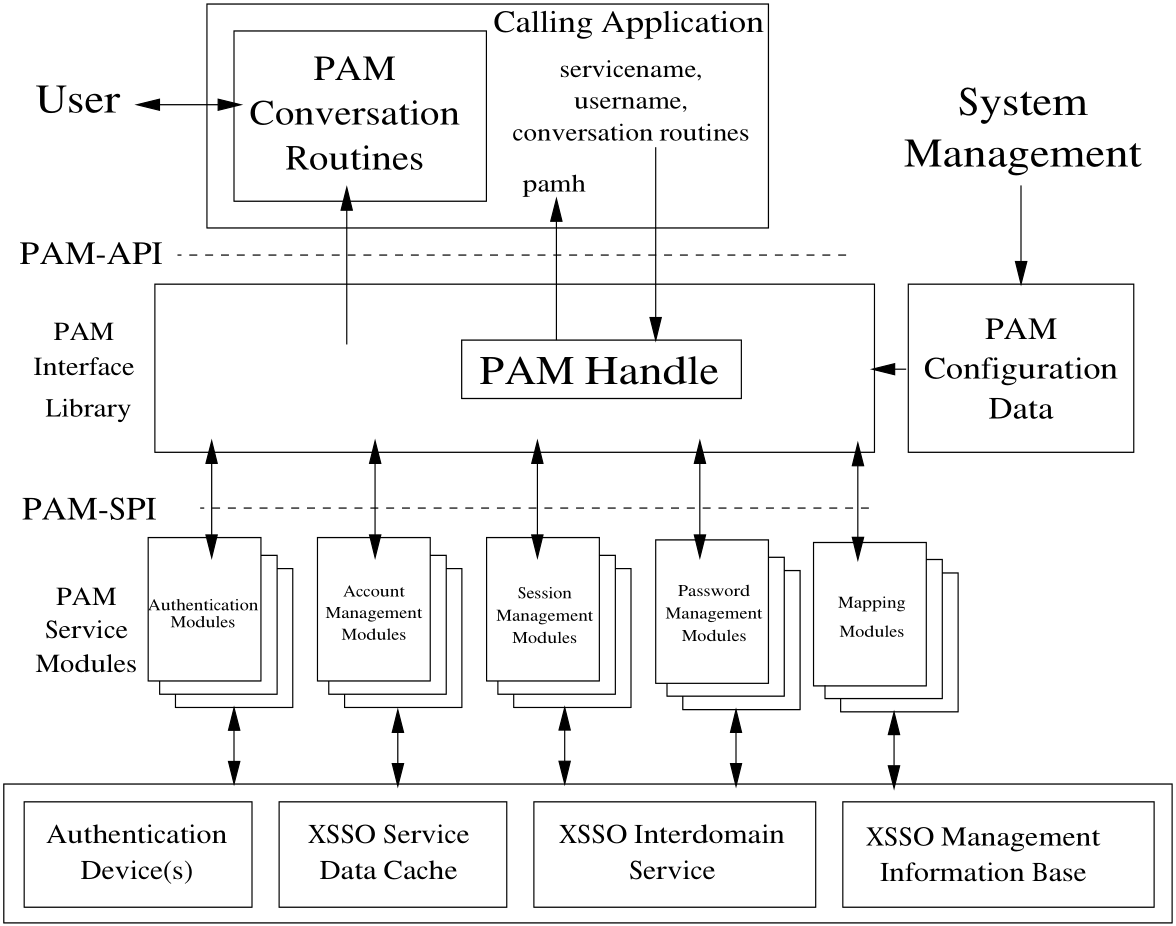
\includegraphics[width=0.8\textwidth]{Media/PAMFramework.png}
    \caption{Arquitectura PAM}
    \label{fig:arquitecturaPAM}
\end{figure}
La figura \ref{fig:arquitecturaPAM} ilustra la relación entre las aplicaciones, la librería \gls{acr-pam} y los módulos de autenticación, gestión de cuenta, gestión de sesión y gestión de contraseña. Cuando una aplicación llama a la \gls{acr-api} de \gls{acr-pam}, ésta carga el módulo correspondiente (definido en el archivo de configuración del servicio). La petición inicial se envía al módulo cargado para que realice la operación deseada. Una vez realizada la operación, la capa PAM devuelve la respuesta del módulo de autenticación a la aplicación\cite{PAM}.
\subsubsection{Archivos de configuración}
Por defecto, el framework lee los archivos de configuración de /etc/pam.d/. Si no se encuentra el directorio, se usará el archivo /etc/pam.conf aunque este método está deprecado. Cada servicio tiene su propio archivo. Aunque varias aplicaciones puedan usar el mismo servicio, por ejemplo varias aplicaciones de bloqueo de pantalla pueden usar el servicio \textit{screenLock}, lo estándar es que cada aplicación cree un servicio propio. Estas aplicaciones se deben encargar de crear el servicio y colocarlo en el directorio.
Estos archivos siguen la siguiente estructura:
\begin{lstlisting}
interfaz_modulo	control	nombre_modulo	argumentos_modulo
\end{lstlisting} \par
El campo \textit{interfaz\_módulo} puede tener cuatro tipos, cada uno de estos pertenece a un tipo de proceso de autorización distinto.
\begin{itemize}
	\item{\textit{auth: }}Este módulo autentica a los usuarios. Por ejemplo: Pide y verifica la contraseña del usuario.
	\item{\textit{account: }}Verifica que se permita el acceso. Por ejemplo: Comprueba si se permite iniciar sesión a un usuario a una hora del día.
	\item{\textit{password: }}Cambia la contraseña del usuario.
	\item{\textit{session: }}Configura y gestiona las sesiones de los usuarios. Por ejemplo: Monta la partición del usuario en el directorio \$home.
\end{itemize} \par
El siguiente campo, \textit{control} indica a PAM que hacer con el resultado recibido. Hay varios tipos de control:
\begin{itemize}
	\item{\textit{required: }}Para que el usuario consiga autenticarse, el módulo debe devolver una respuesta positiva. Si el módulo devuelve una respuesta negativa, no se le notifica al usuario hasta que se acaben de pasar todos los módulos.
	\item{\textit{requisite: }}Para que el usuario consiga autenticarse, el módulo debe devolver una respuesta positiva. Si el test falla, se avisa al usuario inmediatamente después de la ejecución del módulo.
	\item{\textit{sufficient: }}Si el módulo devuelve un resultado negativo, éste se ignora. Si ningún módulo previo \textit{required} ha fallado, no son necesarios más módulos para autenticar correctamente al usuario.
	\item{\textit{optional: }}Se ignora su resultado. Solo se necesita para autenticar al usuario si ningún otro módulo referencia la interfaz.
	\item{\textit{include: }}Referencia todas las líneas del archivo especificado.
\end{itemize} \par
El tercer campo del archivo, \textit{nombre\_módulo}, proporciona a PAM el nombre del módulo que contiene la interfaz del módulo. No es necesario poner una ruta absoluta al archivo si éste está en el directorio por defecto. \par
El último argumento, \textit{argumentos\_módulo} proporciona al módulo de autenticación los argumentos necesarios para su correcto funcionamiento. \par
Se muestra un ejemplo de este documento en la figura \ref{fig:archivoServicio}.
\begin{figure}[H]
    \centering
    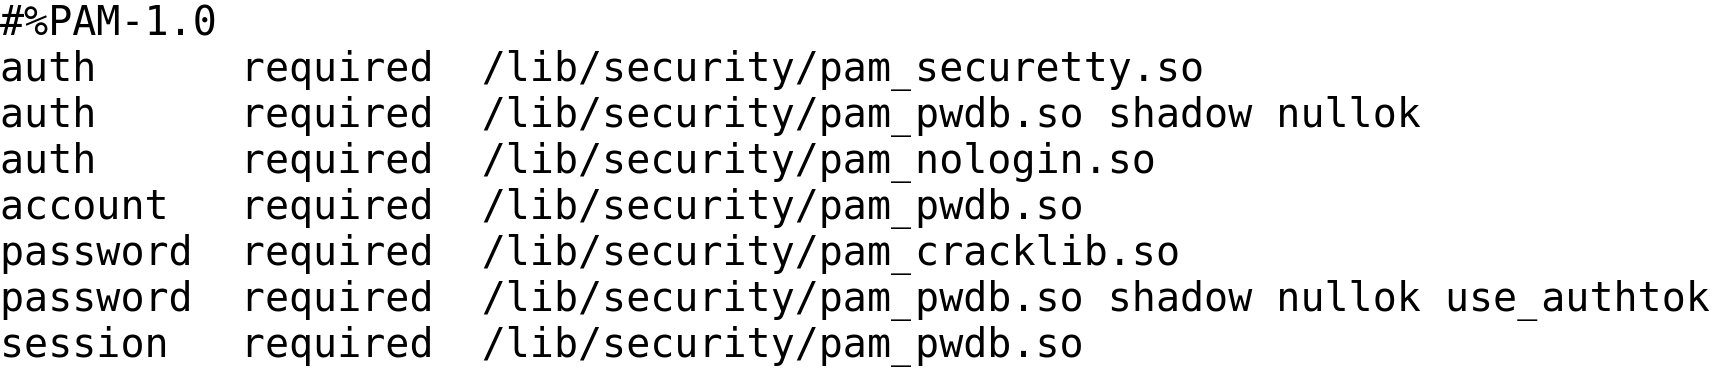
\includegraphics[width=0.7\textwidth]{Media/PAMConfigFile.png}
    \caption{Archivo de configuración de un servicio de ejemplo}
    \label{fig:archivoServicio}
\end{figure}
La primera línea es un comentario. Cualquier línea que empiece por (\#) es un comentario. Los módulos de autenticación son las líneas 2, 3 y 4. El módulo
\begin{lstlisting}
auth required /lib/security/pam_securetty.so
\end{lstlisting}
asegura que, si un usuario está intentando autenticarse como root, el \gls{tty} desde el cual se está autenticando está en el archivo /etc/securetty. Si no está el \gls{tty} ahí, cualquier intento de inicio de sesión como usuario \gls{root} fallará con un mensaje de login incorrecto. \par
El módulo 
\begin{lstlisting}
account required /lib/security/pam_pwdb.so
\end{lstlisting}
comprueba la expiración de un usuario. Si la cuenta ha expirado o la contraseña ha expirado y el usuario no introduce la nueva, el módulo fallará. \par
El módulo 
\begin{lstlisting}
password required /lib/security/pam_pwdb.so shadow nullok use_authtok
\end{lstlisting}
Llama otra vez a \textit{pam\_pwdb} para cambiar la contraseña del usuario en caso de que la haya cambiado. Los argumentos le indican a módulo que escriba las contraseñas en \textit{shadow}, que acepte una contraseña en blanco como válida y que use la nueva contraseña, en caso de que se haya cambiado. \par
El módulo
\begin{lstlisting}
session required /lib/security/pam_pwdb.so
\end{lstlisting}
se encarga de guardar en el log del sistema el inicio de sesión. Si la operación no se consigue realizar, el usuario no podrá iniciar sesión en el sistema.
\subsubsection{PAM-API}
El proceso de autenticación lo gestiona la librería PAM via una llamada a la función \textit{pam\_authenticate()}. El valor devuelto por esta función determinará si el usuario ha sido autenticado. Si la librería PAM debe preguntarle al usuario por la contraseña o su nombre de usuario, lo hará. Si la librería PAM autentica mediante el uso de un protocolo silencioso, también lo hará. (Un dispositivo hardware por ejemplo)\cite{linux-pam-application} \par
Las funciones más importantes para nuestra interfaz de módulo (auth) de la \gls{acr-api} PAM son:
\begin{lstlisting}
#include <security/pam_appl.h>
const char* nombre_servicio;
const char* usuario;
const struct pam_conv* conversacion_pam;
pam_handle_t** gestor_pam;

int pam_start(nombre_servicio, usuario, conversation_pam, gestor_pam);
\end{lstlisting}
La primera función a la que se tiene que llamar es a \textit{pam\_start()}. Esta crea el contexto PAM e inicializa la transacción PAM.\par
\begin{itemize}
	\item{\textit{nombre\_servicio}: Especifica el nombre del servicio que usar. Se leerá el contenido del servicio de /etc/pam.d/\textit{nombre\_servicio}}
	\item{\textit{usuario}: Especifica el nombre de usuario. Si es \textit{null}, el módulo se encarga de solicitarlo si es necesario}
	\item{\textit{conversacion\_pam}: Apunta a una estructura de tipo \textit{pam\_conv} que describe la función de conversación a usar.}
	\item{\textit{gestor\_pam}: Dada una respuesta correcta (PAM\_SUCCESS) \textit{gestor\_pam} contiene el contexto necesario para próximas peticiones a funciones PAM.}
\end{itemize} 
Esta función devuelve:
\begin{itemize}
	\item{PAM\_ABORT: fallo general}
	\item{PAM\_BUFF\_ERR: Error en el buffer de memoria}
	\item{PAM\_SUCCESS: Transacción creada correctamente}
	\item{PAM\_SYSTEM\_ERR: Error del sistema}
\end{itemize} \par
La última función a la que se tiene que llamar es a \textit{pam\_end}. Invalida \textit{gestor\_pam}. A partir de este momento, ya no se podrá usar para interaccionar con la \gls{acr-api} PAM.
\begin{lstlisting}
#include <security/pam_appl.h>
pam_handle_t* gestor_pam;
int estado_pam;

int pam_end(gestor_pam, estado_pam);
\end{lstlisting}
\begin{itemize}
	\item{\textit{gestor\_pam}: Estructura que identifica la operación con la \gls{acr-api} PAM.}
	\item{\textit{estado\_pam}: El estado devuelto por el último método PAM. Se le pasa a la función \textit{cleanup()} para que ésta gestione debidamente la liberación de los datos.}
\end{itemize}
Esta función devuelve:
\begin{itemize}
	\item{PAM\_SUCCESS: Transacción creada correctamente}
	\item{PAM\_SYSTEM\_ERR: Error del sistema}
\end{itemize} \par
PAM también proporciona funciones para acceder y actualizar información PAM. Para esto, hace uso de funciones getter y setter. Estas dos son \textit{pam\_set\_item()} y \textit{pam\_get\_item()}.
La función setter:
\begin{lstlisting}
#include <security/pam_modules.h>
pam_handle_t* gestor_pam;
int tipo_de_dato;
const void* dato;

int pam_set_item(gestor_pam, tipo_de_dato, dato);
\end{lstlisting}
La función getter:
\begin{lstlisting}
#include <security/pam_modules.h>
pam_handle_t* gestor_pam;
int tipo_de_dato;
const void** dato;

int pam_get_item(gestor_pam, tipo_de_dato, dato);
\end{lstlisting}
A estas dos funciones se les pasan:
\begin{itemize}
	\item{\textit{gestor\_pam}: Estructura que identifica la operación con la \gls{acr-api} PAM.}
	\item{\textit{tipo\_de\_dato}: Indica el tipo de dato que va a leer a continuación. Pueden ser: PAM\_SERVICE, PAM\_USER, PAM\_TTY entre otros}
	\item{\textit{dato}: Dato a cambiar o obtener de PAM}
\end{itemize}
\textit{pam\_set\_item()} devuelve:
\begin{itemize}
	\item{PAM\_BAD\_ITEM: Se ha intentado asignar un valor inaccesible.}
	\item{PAM\_BUFF\_ERR: Error en el buffer de memoria}
	\item{PAM\_SUCCESS: Transacción creada correctamente}
	\item{PAM\_SYSTEM\_ERR: Error del sistema}
\end{itemize} 
\textit{pam\_get\_item()} devuelve:
\begin{itemize}
	\item{PAM\_BAD\_ITEM: Se ha intentado obtener un valor inaccesible.}
	\item{PAM\_BUFF\_ERR: Error en el buffer de memoria}
	\item{PAM\_PERM\_DENIED: El valor del dato era \textit{null}.}
	\item{PAM\_SUCCESS: Transacción creada correctamente}
	\item{PAM\_SYSTEM\_ERR: Error del sistema}
\end{itemize} 
\textit{pam\_authenticate()} es la función más importante de la \gls{acr-api} , ya que todo gira en torno a esta. Al haber preparado todo anteriormente con la función \textit{pam\_start()} esta función es bastante sencilla de entender.
\begin{lstlisting}
#include <security/pam_appl.h>
pam_handle_t* gestor_pam;
int flags;

int pam_authenticate(gestor_pam, flags);
\end{lstlisting}
A esta función se le pasan los argumentos:
\begin{itemize}
	\item{\textit{gestor\_pam}: Estructura que identifica la operación con la \gls{acr-api} PAM.}
	\item{\textit{flags:} Pueden ser dos:
		\begin{itemize}
			\item PAM\_SILENT: no registra ningún mensaje.
			\item PAM\_DISALLOW\_NULL\_AUTHTOK: Si el usuario no tiene un token de autenticación registrado, hace que el módulo devuelva PAM\_AUTH\_ERR}
		\end{itemize} 
\end{itemize}
\textit{pam\_authenticate()} devuelve:
\begin{itemize}
	\item{PAM\_ABORT: Aplicación deberá salir inmediatamente}
	\item{PAM\_AUTH\_ERR: Usuario no autenticado}
	\item{PAM\_CRED\_INSUFFICIENT: Aplicación no tiene suficiente información para autenticar al usuario}
	\item{PAM\_AUTHINFO\_UNVALID: Módulos han sido incapaces de acceder a la información de autenticación}
	\item{PAM\_MAXTRIES: Uno o más módulos han llegado al límite de intentos. No volver a intentar}
	\item{PAM\_SUCCESS: Usuario satisfactoriamente autenticado}
	\item{PAM\_USER\_UNKNOWN: Usuario no reconocido}
\end{itemize}
Existen varias funciones más en la \gls{acr-api}, que son esenciales para la gestión de las otras interfaces de módulo pero para entender PAM y el módulo \textit{auth} no son necesarias.\par
\textit{pam\_conv} no es una función, sino una estructura que permite al módulo y a la aplicación que le ha llamado comunicarse directamente.
\begin{lstlisting}
struct pam_conv{
    int (*conversacion) (int, struct pam_mensaje **,
          struct pam_respuesta **, void *appdata_ptr);
    void *appdata_ptr;
};
\end{lstlisting}
donde \textit{conversacion} es:
\begin{lstlisting}
int conversacion(int numero_mensajes, const struct pam_message **mensaje,
		 struct pam_response **respuesta, void *appdata_ptr);
\end{lstlisting}
Generalmente se usa para mostrar y recibir información del usuario. Se especifica cuando se llama a \textit{pam\_start()} al iniciar el procedimiento. Esta estructura debe tener dos elementos para ser válida:
\begin{itemize}
	\item{Función de conversación pasada por referencia}\par Un puntero a la función de conversación. Esta función es la que gestiona la comunicación entre el módulo y la aplicación.
	\item{\textit{void* appdata\_ptr}}\par
		Al pasarse mediante la función de conversación al módulo y ser devuelta por el mismo, la aplicación puede usar este campo para pasar información específica de la aplicación al módulo.
\end{itemize}
\subsubsection{PAM-SPI}
Igual que la \gls{acr-api}, la \gls{acr-spi} proporciona funciones para poder gestionar los cuatro pilares del módulo PAM (\textit{authentication}, \textit{account}, \textit{session} y \textit{password}) pero nosotros nos vamos a centrar en las funciones necesarias para la parte de \textit{authentication}. El proceso de verificación se gestiona con la función \textit{pam\_sm\_authenticate()}.
\begin{lstlisting}
#define PAM_SM_AUTH
#include <security/pam_modules.h>
pam_handle_t* gestor_pam;
int flags;
int argc;
const char** argv;

PAM_EXTERN int pam_sm_authenticate(gestor_pam, flags, argc, argv);
\end{lstlisting}
Se usa \textit{PAM\_SM\_AUTH} para asegurar que los prototipos de los módulos estáticos estén bien declarados.
Los parámetros que se le pasan a \textit{pam\_sm\_authenticate()} son: 
\begin{itemize} 
	\item \textit{gestor\_pam}: Estructura que identifica la operación con la \gls{acr-api} PAM.
	\item{\textit{flags:} Pueden ser dos:
		\begin{itemize}
			\item PAM\_SILENT: no registra ningún mensaje.
			\item PAM\_DISALLOW\_NULL\_AUTHTOK: Si el usuario no tiene un token de autenticación registrado, hace que el módulo devuelva PAM\_AUTH\_ERR}
		\end{itemize} 
	\item{\textit{argc} y \textit{argv}: Funcionan como el paso de parámetros a una función estándar en \gls{C}.
\end{itemize}
\textit{pam\_sm\_authenticate()} devuelve:
\begin{itemize}
	\item{PAM\_AUTH\_ERR: Usuario no autenticado}
	\item{PAM\_CRED\_INSUFFICIENT: Aplicación no tiene suficiente información para autenticar al usuario}
	\item{PAM\_AUTHINFO\_UNVALID: Módulos han sido incapaces de acceder a la información de autenticación}
	\item{PAM\_MAXTRIES: Uno o más módulos han llegado al límite de intentos. No volver a intentar}
	\item{PAM\_SUCCESS: Usuario satisfactoriamente autenticado}
	\item{PAM\_USER\_UNKNOWN: Usuario no reconocido}
\end{itemize}
Aunque esta sea la única función necesaria para implementar el módulo \textit{authentication}, existen varias funciones que ayudan a la implementación de esta función como \textit{pam\_get\_user()} o \textit{pam\_get\_item()}. La segunda está descrita en la sección superior.
\begin{lstlisting}
#include <security/pam_modules.h>
pam_handle_t** gestor_pam;
const char** usuario;
const char* avisoUsuario;

int pam_get_user(gestor_pam, user, prompt);
\end{lstlisting} 
\textit{pam\_get\_uer()} se usa para obtener el usuario que está solicitando la autenticación. Devuelve el nombre del usuario especificado por \textit{pam\_start()}. Si no se especificó ningún usuario, se devuelve el valor de \textit{pam\_get\_item(gestor\_pam, PAM\_USER, ...)}. Si este valor es \textit{null}, averigua el usuario mediante \textit{pam\_conv()}.
\begin{itemize}
	\item \textit{gestor\_pam}: Estructura que identifica la operación con la \gls{acr-api} PAM.
	\item \textit{usuario}: Se devuelve un puntero a \textit{user}. El valor del usuario no se debería liberar ni modificar.
	\item \textit{prompt}: Diálogo que se le presenta al usuario al pedirle la contraseña.
\end{itemize}
Los valores de retorno de esta función son:
\begin{itemize}
	\item{PAM\_SUCCESS: Nombre de usuario devuelto satisfactoriamente.}
	\item{PAM\_SYSTEM\_ERROR: Puntero a \textit{null} pasado por parámetros}
	\item{PAM\_CONV\_ERROR: La función de conversación proporcionada por la aplicación no obtuvo un nombre de usuario.}
\end{itemize}
\subsubsection{Módulos \gls{acr-dfa} para \gls{acr-pam}}
Existen varios módulos que utilizan PAM para realizar el proceso de autorización del usuario. Cada uno proporciona al usuario distintas cualidades.
\begin{itemize}
	\item{Google Authenticator}\par
	Este\footnote{\url{https://github.com/google/google-authenticator-libpam}} módulo usa \gls{acr-otp} como sistema para verificar la autenticidad del usuario.
	\item{pam\_geoip}\par
	Este\footnote{\url{http://ankh-morp.org/code/pam_geoip/}} módulo autentica al usuario según la zona geográfica en la que se encuentre el sistema.
	\item{pam-face-authentication} \par
	Este\footnote{\url{https://code.google.com/archive/p/pam-face-authentication/}} módulo autentica al usuario mediante un escaneo de sus rasgos faciales.
	\item{poldi} \par
	Este\footnote{\url{http://www.g10code.com/p-poldi.html}} módulo autentica al usuario mediante una tarjeta inteligente.
\end{itemize}
\subsubsection{Un entorno \gls{acr-pam}, uniéndolo todo}
A pesar de ser un sistema más convencional de autenticación, se decidió crear un módulo \gls{acr-usb} porque la disponibilidad de tarjetas inteligentes o aplicaciones de autenticación es inferior a la de \gls{acr-usb}s. Además, cualquier persona posee un \gls{acr-usb} hoy en día. Esto acerca más el \gls{acr-dfa} a los usuarios. \par
Al ya existir un módulo\footnote{\url{https://github.com/ColumPaget/pam_usbkey}} \gls{acr-dfa} por \gls{acr-usb}, se decidió no reinventar la rueda y ayudar de otra forma a la comunidad. Aún así, se explicarán los pasos necesarios para la creación de dicho módulo. \par
Antes de nada, debemos establecer el papel del \gls{acr-usb} en el módulo. El hecho de que se use un \gls{acr-usb} nos da pié a multitud de opciones. Al ser un dispositivo que el ordenador reconoce sin problemas, podemos interaccionar con el, sin necesidad de descargar e instalar programas que harían la adopción del módulo mucho más nicho.\par
Antes de empezar con el módulo en sí, se debe explicar como se detectan los \gls{acr-usb}'s en el sistema. Se debe entender que antes de que nosotros podamos usar el dispositivo, el sistema debe haberlo reconocido e iniciado un proceso de comunicación entre él mismo y el \gls{acr-usb}. Una vez el \gls{acr-usb} ya está detectado por el sistema, nuestro programa debería funcionar sin problemas.\par
Los \gls{acr-usb}, como cualquier dispositivo hardware tienen grabados unos datos desde fábrica, para identificarlos de forma única. Estos datos son los que usa el módulo para diferenciar entre dispositivos y solo devolver \textit{PAM\_SUCCESS} cuando detecta el indicado.\par
Para crear este módulo, nos aprovecharemos de la \gls{acr-spi} de \gls{acr-pam}. Como ya hemos visto anteriormente, únicamente necesitamos implementar un método, \textit{pam\_sm\_authenticate()}. Este comprueba que el dispositivo \gls{acr-usb} sea el indicado y si lo es, devuelve \textit{PAM\_SUCCESS}. 
Para comprobar el identificador único del \gls{acr-usb} antes debemos proporcionarle al módulo la lista de identificadores que están permitidos. Estos parámetros, además de algunos otros como el usuario, la \gls{acr-tty} y los hosts remotos. Estos parámetros los introduce el administrador de sistema en el campo \textit{argumentos\_modulo} dentro del \textit{service} de la siguiente manera:
\begin{lstlisting}
auth required pam_usbkey.so user=* rhosts=* tty=* key=12345678910
\end{lstlisting}
El módulo los recibe mediante los parámetros \textit{argc} y \textit{argv} de la función \textit{pam\_sm\_authenticate()} y los trata para poder usarlos. Una vez tiene los parámetros, debe comparar de forma no excluyente los datos. En el fragmento superior, los parámetros indican que cualquier usuario, representado por el carácter (*) en cualquier \gls{acr-tty} con cualquier dirección IP puede autenticarse en el módulo si detecta que el identificador \gls{acr-usb} es 12345678910. Tras comparar los parámetros, se ejecuta el siguiente pseudocódigo:
\begin{lstlisting}[xleftmargin=.07\textwidth]
if (UsuarioCoincide && (TTYCoincide || HostCoincide)){
	if (! IdentificadorCoincide) return(PAM_PERM_DENIED);
	return(PAM_SUCCESS);
}
return(PAM_IGNORE);
\end{lstlisting}
Si el usuario coincide y coincide el \gls{acr-tty} o la dirección IP desde la que se conecta el usuario, si no coincide el identificador del \gls{acr-usb} devuelve \textit{PAM\_PERM\_DENIED}. Si el programa aún no ha devuelto nada, significa que si que coincide el identificador así que devuelve \textit{PAM\_SUCCESS}. Si no coincidía el usuario y el \gls{acr-tty} o la dirección IP, devuelve \textit{PAM\_IGNORE}.\par
Para crear una aplicación \textit{pam-aware} debemos usar los métodos de la \gls{acr-api}. Lo primero que debemos hacer es definir nuestra conversación. Esto permite una comunicación directa entre un módulo y una aplicación. En el código de demostración inferior, vemos como se inicializa la estructura.
\begin{lstlisting}[xleftmargin=.1\textwidth]
struct pam_conv conv = {funcion_conversacion, NULL};
\end{lstlisting}
Una vez tenemos eso, debemos inicializar el gestor, este se encarga de identificar el proceso. Esto se hace con el código a continuación.
\begin{lstlisting}[xleftmargin=0\textwidth]
if ((ret = pam_start("bloqueo", usuario, &conv, &gestor_pam) != PAM_SUCCESS)
	errx(EXIT_FAILURE, "PAM: %s", pam_strerror(gestor_pam, ret));
\end{lstlisting}
Llama a \textit{pam\_start()} con los argumentos necesarios descritos anteriormente y controla el valor devuelto englobando la llamada en la condición del \textit{if}. De esta forma, nos aseguramos que si algo sale mal en el proceso, lo tenemos controlado y podemos gestionar el error.\par
Una vez tenemos todo el entorno preparado, podemos hacer uso de la función \textit{pam\_authenticate()}. El resultado de llamar a esta función le dirá a la aplicación si podemos o no iniciar sesión en el sistema. Un ejemplo de implementación:
\begin{lstlisting}[xleftmargin=.07\textwidth]
    if (pam_authenticate(gestor_pam, 0) == PAM_SUCCESS) {
        pam_setcred(gestor_pam, PAM_REFRESH_CRED);
        pam_end(gestor_pam, PAM_SUCCESS);
        ev_break(EV_DEFAULT, EVBREAK_ALL);
        return;
    }
\end{lstlisting}
Una vez entra dentro de la condición el usuario ya ha sido autenticado por \gls{acr-pam}. Lo que queda hacer es preparar todo para que el programa termine correctamente. Estos pasos son: actualizar las credenciales, terminar la comunicación con \gls{acr-pam} y salir del programa.\par
Estas dos implementaciones no van a funcionar entre sí a no ser que el administrador de sistemas las vincule en el archivo de configuración (\textit{service}) del módulo. En este archivo, el administrador de sistemas introducirá la sentencia que une ambas cosas. Como hemos visto anteriormente, un posible ejemplo es:
\begin{lstlisting}
auth required pam_usbkey.so user=* rhosts=* tty=* key=12345678910
\end{lstlisting}
En este caso, se indica que la interfaz del módulo es de autenticación, que el módulo pam\_usbkey.so debe devolver una respuesta positiva. Los parámetros que se le proporciona al módulo son los cuatro de la regla.
\subsection{Pruebas \gls{acr-dfa} desarrolladas según tecnología}
Durante el desarrollo del proyecto he implementado y probado una serie de mecanismos \gls{acr-dfa}. Este es el resumen de estos distintos proyectos, sus problemas y ventajas.
\subsubsection{\gls{dbus}}
El primer proyecto que intenté, \gls{dbus}, esencialmente es algo muy parecido a una autopista para el sistema. A través de él se pueden comunicar todos los programas entre ellos. Esto significa que dependiendo de los métodos disponibles en cada programa, se  podría enviar (mediante un programa que esté a la escucha de una señal) una señal al programa de bloqueo diciéndole que se apague/pare, que el usuario ya está autenticado. Bastantes programas de bloqueo en distribuciones como \gls{Ubuntu} tienen un sistema \gls{dbus} implementado así que merecía la pena probar.\par
Las ventajas de este tipo de sistemas son:
\begin{itemize}
	\item{\textbf{Ligero}}\par
		El programa que yo debía implementar simplemente estaba a la escucha de una señal/patrón constantemente. Cuando lo recibía enviaba un comando al programa de bloqueo, que bloqueaba o desbloqueaba la pantalla del sistema. 
	\item{\textbf{Sencillo de implementar}}\par
		En Python, estamos hablando de aproximadamente 40 líneas de programa.
	\item{\textbf{Silencioso}}\par
		Es perfecto para no dejar rastro en el sistema. Comprobar los logs de \gls{dbus} es como buscar una aguja en un pajar, por ese demonio pasan tantos datos que sería muy poco práctico monitorizarlo. Es perfecto para una puerta trasera en un sistema, pero ese no es mi objetivo.
\end{itemize}
Los inconvenientes de una implementación de este estilo son:
\begin{itemize}
	\item{\textbf{Específico}}\par
		Cada distribución usa un programa de bloqueo de pantalla, esto significa cambiar la lógica del programa cada vez que quiera usarlo en un ordenador distinto al mío.
	\item{\textbf{Ejecución constante}}\par
		Aunque sea ligero, el programa debe estar en constante ejecución. Esto, por poco que sea, consume tiempo de procesamiento del procesador.
	\item{\textbf{No hace uso de las herramientas proporcionadas por \gla{GNU/Linux}}\par
		Este enfoque hacia la autenticación de usuarios no hace uso de las utilidades proporcionadas por \gls{GNU/Linux} para autenticar un usuario.
	\item{\textbf{Difícil de configurar}}\par
		Aunque su implementación es relativamente sencilla, al querer reducir la barrera de entrada del usuario medio a sistemas \gls{acr-dfa}, el proceso de configuración del programa era demasiado complicado. Se tiene que configurar para que se ejecute siempre que se inicia el sistema.
\end{itemize}
Durante una serie de iteraciones de investigación/implementación se continuaron probando programas basados en el mismo principio. Todos ellos se encontraron en \gls{GitHub}. \par
En la primera fase de implementación se creó un script que bloqueaba el ordenador al ejecutarlo. \par
La siguiente fase se dedicó a buscar ejemplos de implementaciones parecidas, para ver como conseguían desbloquear la pantalla mediante dbus. Se encontraron varios proyectos, entre ellos \href{https://github.com/Svenito/usblock}{usblock}. Este proyecto gestionaba el bloqueo/desbloqueo de la pantalla mediante \gls{dbus}, un buen ejemplo de implementación.\par
Al descargar y ejecutar el programa, me encontré con que estaba usando una librería obsoleta. \gls{acr-hal}. Durante un par de semanas se intentó por todos los medios solucionar el problema en cuestión, pero esta librería fue reemplazada por \gls{udev}. Al ver esto, solamente podía leer el programa pero no podía probarlo en mi sistema debido a que \gls{acr-hal} no está presente.\par
Haciendo balanza de las ventajas e inconvenientes, se decidió buscar una solución distinta.\par
\subsubsection{\gls{acr-pam}}
La siguiente tecnología que encontré fue \gls{acr-pam}. Esta vez, aseguré que era exactamente lo que necesitaba ya que no quería perder más tiempo probando e intentando arreglar cosas que no tenían sentido. Al investigar más a fondo los distintos tipos de autenticación existentes en \gls{GNU/Linux} y ver que muchos de ellos eran compatibles con \gls{acr-pam}, supe que debía seguir investigando esta tecnología. \par
El primer proyecto que encontré, fue \href{https://github.com/aluzzardi/pam_usb}{PAM\_USB}\footnote{\url{https://github.com/aluzzardi/pam_usb}}. Las siguientes fases de investigación/implementación se dedicaron a investigar y entender este módulo para \gls{acr-pam}. Cabe mencionar que en este momento el desarrollo de un módulo propio para \gls{acr-pam} ya no tenía sentido, ya que un usuario de \gls{GitHub} llamado aluzzardi, el creador del programa había creado un módulo muy bien documentado y programado. Cuando lo descargué para probar y configurar en el sistema, el módulo no detectaba los dispositivos \gls{acr-usb} que conectaba. Tras una investigación, se averiguó que este módulo también usaba \gls{acr-hal} para detectar los dispositivos conectados.\par
Al ser un proyecto popular y usado por la comunidad, se pensó que seguramente existiesen pull requests por miembros de la comunidad para portar el proyecto a \gls{udev}. Efectivamente, si existían. Al descargar y probar este\footnote{\url{https://github.com/aluzzardi/pam_usb/pull/34}} me encontré con que también habían complicaciones. Se proporcionaban una serie de scripts para ayudar con la configuración del módulo. Ambos parecían estar escritos en la versión 2 de Python pero ninguno parecía funcionar en mi sistema.\par Al experimentar esto, cambié de proyecto a uno menos ambicioso. Empecé a usar \href{https://github.com/ColumPaget/pam_usbkey}{pam\_usbkey}\footnote{\url{https://github.com/ColumPaget/pam_usbkey}}. Este módulo, esencialmente hace lo mismo que PAM\_USB pero no tiene tanto nivel de seguridad, ya que comprueba el ID del \gls{acr-usb} pero no una llave firmada dentro del \gls{acr-usb}. \par
Las ventajas de usar módulos para \gls{acr-pam} son:
\begin{itemize}
	\item{\textbf{Integración absoluta con cualquier sistema que use \gls{acr-pam}}}\par
		Al ser un módulo tan extendido, esto significa que prácticamente cualquier usuario de \gls{GNU/Linux} e incluso MacOS puede disfrutar de las ventajas del \gls{acr-dfa}
	\item{\textbf{Ejecución bajo petición}}\par
		El módulo se carga cuando una aplicación solicita que se use dicho módulo para proceder a verificar la identidad del usuario
	\item{\textbf{Versatilidad}}\par
		El programador del módulo puede usar cualquier método imaginable para autenticar al usuario, \gls{acr-pam} ofrece la posibilidad de gestionar todos los módulos por igual.
	\item{\textbf{Configurabilidad}}\par
		El administrador de sistemas puede intercambiar los módulos que va a usar una aplicación de forma muy sencilla.
	\item{\textbf{Configuración centralizada}}\par
		El administrador de sistemas tiene todos los archivos de configuración en un directorio, ordenados según \textit{service}
	\item{\textbf{Facilidad de uso para usuarios no avanzados}}\par
		Un usuario medio puede configurar un módulo \gls{acr-pam} sin mucho problema.
\end{itemize}
Los inconvenientes de \gls{acr-pam} son:
\begin{itemize}
	\item{\textbf{Curva de aprendizaje}}\par
		Aunque sencilla, el programador debe aprender como funciona \gls{acr-pam} para crear un módulo.
\end{itemize}
\subsection{Creación del \gls{script}}
Ésta es la parte práctica, derivada de la parte teórica de este trabajo. El \gls{script} se ha escrito en \gls{acr-bash}. Un lenguaje intérprete de comandos. Esto significa que une distintos programas disponibles, como: \textit{ls, mv, cd, sed} o \textit{cat} para crear un único programa, que cumple una función específica.\par
\subsubsection{Selección del lenguaje}
Se decidió usar \gls{acr-bash} porque está disponible en todos los equipos que usan \gls{acr-pam}, me interesaba aprenderlo inicialmente y la curva de aprendizaje inicial no parecía muy complicada.\par
\subsubsection{Aprendizaje del lenguaje}
Antes de desarrollar el \gls{script}, debía aprender como funcionaba el lenguaje así que busqué un curso on-line para aprender. 
Este\footnote{\url{https://guide.bash.academy/}} curso, casualmente también código abierto a la comunidad, explica los conceptos básicos y las buenas prácticas asociadas al desarrollo de \gls{script}s en \gls{acr-bash}.\par
\subsubsection{Estilo de código}
Durante el desarrollo del \gls{script} he usado la guía de estilos de \href{https://www.google.com}{Google}\footnote{\url{https://google.github.io/styleguide/shell.xml}}. Pienso que ceñirse a un estilo y ser consistente a la hora de programar ayuda enormemente a la comprensión del código.\par
\subsubsection{¿Qué va a solventar?}
El \gls{script} está diseñado para ser de utilidad una vez se consigue instalar el módulo. Una vez hecho eso, se ejecuta el \gls{script} para gestionar la generación de la regla a insertar en el archivo indicado. Este proceso es el más complicado de toda la gestión porque al existir multitud de opciones, el usuario menos experimentado se puede ver inundado entre ellas. El \gls{script} informa en todo momento los pasos que está haciendo y explica que posibles acciones que puede tomar a continuación. \par
La finalidad del \gls{script} es facilitar la configuración de un módulo \gls{acr-pam}.
\subsubsection{Funcionalidad}
El \gls{script}, solo se inicia, informa al usuario que debe tener precaución, ya que una mala configuración puede resultar en un bloqueo permanente de sesión. Tras aceptar las cláusulas, se le pide que introduzca el \gls{acr-usb} que quiere usar como \gls{acr-dfa}. Tras haber introducido el \gls{acr-usb} se le presentan los dispositivos encontrados en el sistema y se le pide que seleccione uno. Al seleccionar uno, se pasa al siguiente paso. En este paso se informa al usuario de las distintas opciones que puede elegir y se le pide que seleccione una. Una vez tenemos la sentencia de configuración, se analiza el archivo en el que se va a insertar y se le muestran al usuario solamente las líneas necesarias con su número de línea. Se le pregunta en que línea quiere poner la regla y verificamos con el usuario. Si todo va bien, se le pregunta una última vez si está seguro de que quiere proceder. Si dice que sí, escribimos la línea en el archivo de configuración. El \gls{script} permite usarse con parámetros para usuarios más avanzados, si no, se usa la configuración por defecto.
\subsubsection{Problemas encontrados durante el desarrollo}
Durante el desarrollo, se han encontrado algunos problemas leves debidos a falta de práctica con el lenguaje. Esto es normal, ya que todos los lenguajes de programación tienen su notación específica.
\subsubsection{Ventajas de usar \gls{acr-bash}}
Durante el desarrollo del \gls{script} ha sido más que evidente el valor que aporta \gls{acr-bash}. El hecho de poder integrar programas específicos en un programa global, permite al programador centrarse en la lógica de la aplicación deseada y delegar la gestión de partes específicas a los programas para completar la tarea.
\clearpage
\section{Conclusiones}
En esta sección, se analizará el desarrollo del proyecto y describirán posibles formas de continuar con él.
\subsection{Conclusiones del proyecto}
Durante el desarrollo del proyecto ha habido veces en las que he sentido que me superaba, que era imposible hacer lo que tenía que hacer y que la mejor estrategia era abandonar y hacer otro trabajo el año que viene. Todas estas, son las fases naturales de un proyecto tan exigente como estimulante. Es importante identificar la parte en la que te encuentras, proceder según el plan y entender que cuando las cosas se vuelven complicadas es que se está explorando más allá de la zona de confort.
Me ha gustado mucho investigar profundamente el funcionamiento de \gls{acr-pam} porque ha hecho que me dé cuenta de que puedo entender y construir software directamente relacionado con algo que uso día a día. Durante la carrera, hemos aprendido a diseñar y construir software, ahora he aprendido a aplicar lo aprendido a un caso de uso real.\par
Como consecuencia del trabajo, al tener que plasmar todo lo aprendido en un lienzo, he tenido que entender perfectamente como funciona la tecnología a explicar. La mejor manera de aprender es explicando.\par
Nunca se nos ha planteado un trabajo tan grande y este está diseñado para afianzar los conocimientos y actitudes desarrolladas durante el periodo de la carrera. En retrospectiva, entiendo y valoro la razón de un trabajo de final de grado ya que enseña a llevar un proyecto de investigación. \par
Finalizando el proyecto, siento que he ampliado mis conocimientos sobre las distintas formas de autenticación y convertido en un experto en \gls{acr-pam}. Esta sensación no la hubiese desarrollado de no ser por este trabajo.\par
En relación al análisis de los sistemas \gls{acr-dfa} puedo concluir en que \gls{acr-pam} al fin y al cabo, no es más que una herramienta para facilitar el desarrollo de buenos sistemas de autenticación. El uso que se le pueda o quiera dar más en adelante depende de cada desarrollador. \par
Está claro que a media que avanzan los tiempos, vamos a tener que inventar nuevas formas de verificar a los usuarios. La belleza de \gls{acr-pam} es que estas nuevas formas se pueden acoplar directamente, como una pieza de lego, en el sistema.\par
Es imposible desarrollar una forma definitiva de verificar al usuario ya que a medida que se desarrollan nuevas, se descubren formas de vulnerarlas. A pesar de las implicaciones negativas que eso conlleva, también incita a la comunidad a desarrollar nuevas y mejores técnicas día a día.
\subsection{Trabajos futuros}
Tras finalizar este trabajo me siento completamente capaz de contribuir a la comunidad haciendo módulos de autenticación para \gls{acr-pam} nuevos. Algunos ejemplos son:
\begin{itemize}
	\item Autenticación mediante huella dactilar
	\item Autenticación mediante escaneo de retina
\end{itemize}
Creo que estos ejemplos serían muy útiles a gente que necesite una mayor seguridad de datos. También puede ser útil a empresas, que quieran centralizar el acceso a áreas restringidas mediante sistemas de autenticación como \gls{acr-pam}.
Debo publicar las partes informativas de este proyecto para asegurar que la gente se pueda beneficiar del trabajo de investigación. Debo subir también el \gls{script} creado a \gls{GitHub} y explicar detalladamente como utilizarlo para acercar más a los usuarios no técnicos esta posibilidad.
\clearpage
\printglossary[type=\acronymtype] %, title={Abreviaciones y tecnicismos}]
\printglossary
\clearpage
\printbibliography[heading=bibintoc,title={Bibliografía}]
\end{document}

